% Preamble
\documentclass[a4paper,14pt]{extarticle}

% Packages
\usepackage{geometry}
\usepackage[T2A]{fontenc}
\usepackage[utf8]{inputenc}
\usepackage[english,russian]{babel}
\usepackage{amsmath}
\usepackage{amsthm}
\usepackage{amssymb}
\usepackage{fancyhdr}
\usepackage{setspace}
\usepackage{graphicx}
\usepackage{colortbl}
\usepackage{tikz}
\usepackage{pgf}
\usepackage{subcaption}
\usepackage{listings}
\usepackage[colorlinks, linkcolor=blue, urlcolor=blue]{hyperref}
\usepackage{indentfirst}

\hypersetup{
    colorlinks=true,
    linkcolor=black,
    urlcolor=blue,
}
\urlstyle{same}
\usepackage{appendix}
\usepackage{algorithm}
\usepackage{amsfonts}
\usepackage{algorithmicx}
\usepackage{algpseudocode}
\usepackage{csquotes}
\usepackage{multirow}
\usepackage{booktabs}
\usepackage{longtable}
\usepackage[sorting=nyt, backend=bibtex]{biblatex}
\addbibresource{bibliography.bib}

\geometry{left=2.5cm}  % левое поле
\geometry{right=1.5cm}  % правое поле
\geometry{top=1.5cm}  % верхнее поле
\geometry{bottom=1.5cm}  % нижнее поле
\renewcommand{\baselinestretch}{1.5}  % междустрочный интервал

\renewcommand{\theenumi}{\arabic{enumi}}  % Меняем везде перечисления на цифра.цифра
\renewcommand{\labelenumi}{\arabic{enumi}}  % Меняем везде перечисления на цифра.цифра
\renewcommand{\theenumii}{.\arabic{enumii}}  % Меняем везде перечисления на цифра.цифра
\renewcommand{\labelenumii}{\arabic{enumi}.\arabic{enumii}.}  % Меняем везде перечисления на цифра.цифра
\renewcommand{\theenumiii}{.\arabic{enumiii}}  % Меняем везде перечисления на цифра.цифра
\renewcommand{\labelenumiii}{\arabic{enumi}.\arabic{enumii}.\arabic{enumiii}.}  % Меняем везде перечисления на цифра.цифра

\DeclareMathOperator*{\argmax}{arg\,max}
\newcommand{\ind}{\hspace{\algorithmicindent}}

\DeclareMathAlphabet{\pazocal}{OMS}{zplm}{m}{n}
\newcommand{\unif}{\pazocal{U}}
\graphicspath{{images/}}

\usepackage{chngcntr}
\counterwithin{figure}{section}
\counterwithin{table}{section}
\counterwithin{algorithm}{section}
\counterwithin{equation}{section}

\makeatletter
\renewcommand*{\@Alph}[1]{\ifcase #1\or А\or Б\or В\or Г\or Д\or Е\or Ж\or З\or И\or К\or Л\or М\or Н\or О\or П\or Р\or С\or Т\or У\or Ф\or Х\or Ц\or Ч\or Ш\or Щ\or Э\or Ю\or Я\else\@ctrerr  \fi}
\makeatother

% Document
\begin{document}

%%%%%%%%%%%%%%%%%%
% ТИТУЛЬНЫЙ ЛИСТ %
%%%%%%%%%%%%%%%%%%
    \thispagestyle{empty}

\textbf{
    \begin{center}
        \small
        Федеральное государственное автономное образовательное учреждение \\
        высшего образования \\
        «Национальный исследовательский университет «Высшая школа экономики»» \\
        Факультет компьютерных наук \\
        Образовательная программа Прикладная математика и информатика \\
        Направление подготовки 01.03.02 Прикладная математика и информатика \\
        бакалавриат
    \end{center}
    \vspace{15pt}
    \begin{center}
        \Large
        ОТЧЕТ \\
        по преддипломной практике
    \end{center}
}
\vspace{15pt}
\textbf{
    \begin{flushright}
        Выполнил студент гр. 171 \\
        Биршерт Алексей Дмитриевич \\
        \makebox[2in]{\hrulefill}
    \end{flushright}
}
\vspace{15pt}
\textbf{
    \begin{flushleft}
        Проверила: \\
        Доцент,\\
        Артемова Екатерина Леонидовна \\
        \makebox[2in]{\hrulefill} \\
        23.04.2021
    \end{flushleft}
}

\vfill
\textbf{
    \begin{center}
        2021 год
    \end{center}
}

%%%%%%%%%%%%%%%%%%
% ТИТУЛЬНЫЙ ЛИСТ %
%%%%%%%%%%%%%%%%%%

    \newpage

%%%%%%%%%%%%%%%%%%
%   ОГЛАВЛЕНИЕ   %
%%%%%%%%%%%%%%%%%%
    {
        \hypersetup{linkcolor=black}
        \tableofcontents
    }
%%%%%%%%%%%%%%%%%%
%   ОГЛАВЛЕНИЕ   %
%%%%%%%%%%%%%%%%%%

    \newpage

%%%%%%%%%%%%%%%%%%
%    АБСТРАКТ    %
%%%%%%%%%%%%%%%%%%
    \begin{abstract}
    В мультиязычных сообществах по всему миру распространён феномен смешения кодов, когда человек использует в речи более одного языка внутри одного предложения.
    Мультиязычные языковые модели показывают впечатляющее качество для разных задач обработки естественного языка.
    Однако реальные данные со смешением кодов очень дороги в сборе и разметке.
    Мы представляем две адверсариальные атаки по методу серого ящика, чтобы оценить возможное качество мультиязычных моделей на входных данных со смешением языков внутри одного предложения.
    Дополнительно мы предлагаем метод адверсариального предобучения для защиты от атак такого рода.
    \parВ своей работе мы решаем задачу одновременного заполнения слотов и распознавания интентов с качеством 98\% accuracy по интентам и 95\% F1 меры по слотам;
    понижаем качество моделей с 78\% до 16\% по метрике semantic accuracy с помощью адверсариальной атаки;
    повышаем качество моделей с 8.8\% до 20\% по метрике semantic accuracy с помощью предложенного метода защиты.
    \newline
    \newline
    Ссылка на гитхаб с проектом - \url{https://github.com/birshert/attack-lang-models}.
    \newline
    \newline
    \textbf{\textit{Ключевые слова---}}Одновременное заполнение слотов и распознавание интентов, адверсариальные атаки, мультиязычные языковые модели, адверсариальное обучение
    \newpage
    There is a common phenomenon in multilingual societies all around the world code-mixing, it consists in mixing different languages inside one utterance.
    Multilingual models have demonstrated incredible performance in various natural language processing tasks.
    However, real code-mixing data is very expensive to collect and label.
    We present two gray-box adversarial attacks, build to evaluate multilingual language models capacity to work with code-mixing input data.
    Additionally we present an adversarial pretraining method to make the models more robust to attacks.
    \par In our work we solve the joint slot-filling and intent recognition task with 98\% intent accuracy and 95\% slots F1 score;
    bring models performance down from 78\% to 16\% in semantic accuracy metric with adversarial attack;
    increase models performance from 8.8\% to 20\% in semantic accuracy metric with proposed protection method.
    \newline
    \newline
    Github project link - \url{https://github.com/birshert/attack-lang-models}.
    \newline
    \newline
    \textbf{\textit{Keywords---}}Joint slot-filling and intent recognition, adversarial attacks, multilingual language models, adversarial training
\end{abstract}

%%%%%%%%%%%%%%%%%%
%    АБСТРАКТ    %
%%%%%%%%%%%%%%%%%%

    \newpage

%%%%%%%%%%%%%%%%%%
%    ВВЕДЕНИЕ    %
%%%%%%%%%%%%%%%%%%


    \section{Введение}
    Последние несколько лет стали прорывными в области мультиязычных моделей и их обобщающей способности для других языков~\cite{Conneau2020UnsupervisedCR,devlin-etal-2019-bert,Liu2020WhatMM,Wu2019BetoBB}.
Огромные мультиязычные модели выучивают универсальные языковые представления, что помогает им демонстрировать удивительные способности к переносу знаний с одного языка на другой.
Простое дообучение предобученных моделей для какой-либо задачи на языке с большим количеством данных позволяет достичь хорошего качества на других языках.
\parОднако простой перенос между языками недостаточен для систем обработки естественного языка для понимания мультиязычных пользователей.
Во многих сообществах в мире достаточно часто явление смешения кодов.
Смешение кодов — это процесс, когда человек спонтанно смешивает различные языки внутри одного предложения или фразы.
Такой феномен может проявляться как в письменной, так и в устной речи.
Таким образом, важно сделать языковую модель устойчивой к смешению языков, чтобы модель адекватно работала со входными данными.
\parНесмотря на то, что реальные данные со смешением кодов очень важны для оценки качества языковых моделей, такие данные очень тяжело собирать и размечать в большом количестве.
\parВ своей работе мы предполагаем, что качество моделей на адверсариальных атаках может служить нижней оценкой на реальное качество модели.
Если языковая модель успешно справляется с адверсариальными пертурбациями со смешением кодов, то и в реальной жизни она будет успешно обрабатывать данные от мультиязычных пользователей.
\parВ своей работе мы:
\begin{itemize}
    \item Решаем задачу одновременного детектирования намерений пользователя и заполнения слотов для диалоговых помощников с помощью мультиязычных языковых моделей.
    \item Предлагаем две адверсариальные атаки по методу серого ящика — во время атаки мы имеем доступ к ошибке модели на заданных данных.
    Насколько нам известно, это одни из первых мультиязычных адверсариальных атак для вышеописанной задачи.
    \item Предлагаем метод адверсариального предобучения.
\end{itemize}
\parВ результате работы мы ожидаем получить следующие результаты:
\begin{itemize}
    \item Мультиязычные модели обучены решать задачу заполнения слотов и классификации интентов.
    \item Проведены две адверсариальные атаки на каждую модель и замерено качество моделей на адверсариальных данных.
    \item Оценено влияние метода адверсариального предобучения на качество моделей на тестовой выборке и после адверсариальных атак.
\end{itemize}
\parВсе свои эксперименты мы будем проводить с современными мультиязычными моделями - m-BERT~\cite{devlin-etal-2019-bert} и XLM-RoBERTa~\cite{Conneau2020UnsupervisedCR}.
В качестве датасета мы будем использовать корпус MultiAtis++~\cite{Xu2020EndtoEndSA}.
\parАктуальность темы подтверждается повышенным интересом со стороны научного сообщества.
После начала работы над исследованием вышло как минимум две статьи на эту тему — в середине марта 2021 года~\cite{Krishnan2021MultilingualCF,Tan2021CodeMixingOS}.

%%%%%%%%%%%%%%%%%%
%    ВВЕДЕНИЕ    %
%%%%%%%%%%%%%%%%%%

    \newpage

%%%%%%%%%%%%%%%%%%
%   ОБЗОР ЛИТРЫ  %
%%%%%%%%%%%%%%%%%%


    \section{Обзор литературы}
    \subsection{Мультиязычные модели}
Языки с небольшим количеством данных часто не могут предоставить достаточного размера датасета для обучения с учителем.
Существует подход для борьбы с этим, который заключается в построении кросс-язычных представлений.
Эти представления нужно дообучать для специфичной задачи на языке с большим количеством ресурсов, чтобы показывать хорошее качество на других, менее ресурсоёмких языках~\cite{klementiev-etal-2012-inducing}.
\parВслед за успехом модели Трансформер~\cite{Vaswani2017AttentionIA},
недавние мультиязычные модели такие как m-BERT~\cite{devlin-etal-2019-bert} и XLM-RoBERTa~\cite{Conneau2020UnsupervisedCR}
переносят парадигму <<предобучение $\rightarrow$ дообучение под специфическую задачу>> в мультиязычную область.
Они предобучают энкодеры на основе архитектуры Трансформера на текстовых данных с различными задачами языкового моделирования.
Затем эти предобученные энкодеры могут быть дообучены для конкретной задачи на ресурсоёмком языке для которого есть много размеченных данных.
Это известно как кросс-язычный перенос знаний.
\parВ одних недавних исследованиях кросс-язычного переноса знаний было показано, что качество модели на ранее не виденных тестовых языках сильно зависит от количества обучающих данных и размера контекста~\cite{Liu2020WhatMM}.
В~\cite{Wu2019BetoBB} было показано, что m-BERT показывает очень сильную способность к кросс-язычному переносу знаний.
m-BERT превосходит по качеству мультиязычные эмбеддинги в четырёх из пяти исследуемых задач без какой-либо информации о связи языков.
\par Более современная и более сложная модель XLM-RoBERTa~\cite{Conneau2020UnsupervisedCR} показывает лучшее, чем m-BERT качество, однако требует массивных объемов обучающих данных для хорошей работы.
В своём исследовании авторы XLM-RoBERTa показывают, что их модель является самой сильной мультиязычной моделью на текущий момент.
\par m-BERT обучается на корпусах Wikipedia и Books, в то время как XLM-RoBERTa обучается на CommonCrawl, который содержит для многих языков на несколько порядков больше данных.

\subsection{Классификация интентов и заполнение слотов}
Повсеместное использование виртуальных ассистентов постепенно становится ежедневной реальностью с ростом их популярности.
Богатство возможностей и качество работы ассистента напрямую влияет на удобство его использования.
Хорошие ассистенты будут привлекать всё больше людей, занимая доли рынка.
Ключевым аспектом в работе виртуального помощника является правильная классификация интентов и заполнение слотов в запросах.
Интент — это желаемый результат запроса пользователя.
Слоты — это слова или наборы слов, которые содержат релевантную интенту информацию.
\parИз-за тесной корреляции между задачами заполнения слотов и классификации интентов обычно используется одна модель для одновременного решения обеих задач~\cite{Weld2021ASO}.
Актуальные подходы последнего времени используют модели на основе Трансформера, например BERT~\cite{devlin-etal-2019-bert}.
Одним из популярных датасетов для этой задачи является датасет MultiAtis++~\cite{Xu2020EndtoEndSA}.

\subsection{Смешение кодов в адверсариальных атаках на мультиязычные модели}
Первые статьи в тематике адверсариальных атак с использованием смешения кодов на мультиязычные модели, такие как m-BERT~\cite{devlin-etal-2019-bert}, Unicoder~\cite{huang-etal-2019-unicoder} и XLM-RoBERTa~\cite{Conneau2020UnsupervisedCR} вышли в середине апреля 2021 года.
В своей работе мы опирались и рассматривали две такие статьи - ~\cite{Tan2021CodeMixingOS} и~\cite{Krishnan2021MultilingualCF}.
\parПервое исследование~\cite{Tan2021CodeMixingOS} посвящено анализу качества моделей m-BERT, Unicoder и XLM-RoBERTa на датасете XNLI под влиянием адверсариальных атак.
В своей работе авторы анализируют две адверсариальные атаки, одна word-level (замена слов в предложении на их эквиваленты из набора языков), вторая phrase-level (замена частей предложения с помощью построения выравниваний).
Так же авторы предлагают метод адверсариального предобучения, который заключается в генерации дополнительных адверсариальных пертурбаций для обучающей выборки и обучения на ней.
\parВторое исследование~\cite{Krishnan2021MultilingualCF} посвящено анализу метода аугментации данных для задачи заполнения слотов и классификации предложений.
В своей работе авторы ставят перед собой цель улучшить перенос знаний на новый неизвестный язык для мультиязычной языковой модели.
Аналогично первой статье, во втором исследовании анализ сконцентрирован на качестве моделей после аугментирования тренировочных данных с помощью смешения кодов.
Авторы предлагают метод chunk-level атаки, которая заключается в сегментации предложений по спанам слотов и замене соответствующих одинаковых сегментов между предложениями на разных языках.
С помощью такой атаки они атакуют обучающую выборку датасета MultiAtis++~\cite{Xu2020EndtoEndSA} и добавляют полученную адверсариальную выборку к исходной обучающей выборке.
\parВ первой статье было установлено, что проведенные адверсариальные атаки очень сильно ухудшили качество мультиязычных языковых моделей.
В первую очередь это может быть связано с тем, что датасет XNLI сам по себе является сложным датасетом и изначальное качество моделей не высоко.
С другой стороны стоит отметить, что в адверсариальных атаках из этого исследования использовалась схема <<один основной язык, много встраиваемых языков>>.
В то время как эта схема не может отражать реалистичные данные со смешением кодов, так как большинство людей, которые могут смешивать коды в речи или на письме, билингвы~\cite{bilinguals}.
\parВо второй статье было установлено, что добавление аугментированных данных в обучающую выборку приводит к улучшению качества для модели m-BERT\@.
Использование дополнительных данных положительно повлияло на низкоресурсные языки.
Так же это положительно сказалось на качестве на языках с отличными от английского морфологическими структурами — китайским и японским.

\subsection{Машинный перевод и выравнивание слов}
Для машинного перевода в своей работе мы будем использовать~\cite{Fan2020BeyondEM}.
Созданная авторами статьи модель обучалась на внушительном датасете из 7.5 миллиардов предложений для 100 языков.
Данная модель основна на архитектуре Трансформера и способна переводить с любого на любой язык в пределе ста обучающих.
На текущий момент это одна из самых сильных моделей для машинного перевода, которая успешно справляется с переводом на любые, даже ранее низкоресурсные, языки.
\parДля построения выравниваний между параллельными предложениями на разных языках мы будем использовать~\cite{Dou2021WordAB}.
Оригинальный подход авторов статьи использует эмбеддинги от мультиязычной языковой модели m-BERT~\cite{devlin-etal-2019-bert}.
Среди результатов постулируется превосходство данного подхода над всеми остальными на текущий момент.

%%%%%%%%%%%%%%%%%%
%   ОБЗОР ЛИТРЫ  %
%%%%%%%%%%%%%%%%%%

    \newpage

%%%%%%%%%%%%%%%%%%
% ОСНОВНАЯ ЧАСТЬ %
%%%%%%%%%%%%%%%%%%


    \section{Основная часть}
    \newcommand{\ind}{\hspace{\algorithmicindent}}

\subsection{Общий вид атаки}

\begin{algorithm}
    \caption{Adversarial attack}
    \begin{algorithmic}
        \Require{Пара пример-метка $x, y$; целевая модель $\mathcal{M}$; набор встраиваемых языков $\mathbb{L}$}
        \Ensure{Адверсариальный пример $x'$} \\
        $\mathcal{L}_{x} = GetLoss(\mathcal{M}, x, y)$
        \For{i in permutation(len(x))}
            \\
            \ind Candidates, Losses = GetCandidates($\mathcal{M}, x, y$, token\_id = i)
            \ind\If{Candidates is not None and max(Losses) > $L_{x}$}
                    \\
                    \ind\ind$L_{x}$ = max(Losses) \\
                    \ind\ind x[i] = Candidates[argmax(Losses)]
            \EndIf
        \EndFor \\
        \Return $x$
    \end{algorithmic}\label{alg:algorithm}
\end{algorithm}

\subsection{Первый метод - word level attack}
В качестве первой атаки была выбрана атака на уровне слов
по аналогии с атакой PolyGloss из ~\cite{Tan2021CodeMixingOS}.
Для перевода используются словари из статьи ~\cite{Choe2020word2wordAC}.

\begin{algorithm}
    \caption{Word-level attack}
    \begin{algorithmic}
        \Require{Набор словарей с исходного на встраиваемые языки $\mathbb{T}$}
        \Function{GetCandidates}{$\mathcal{M}, x, y$, token\_id}
            \\
            \ind Candidates, Losses = [~], [~]\\
            \ind$x_c$ = copy($x$)
            \For{language in $\mathbb{L}$}
                \ind\If{x[token\_id] in $\mathbb{T}$[language]}
                        \\
                        \ind\ind\ind token = $\mathbb{T}$[language][x[token\_id]]\\
                        \ind\ind\ind Candidates.append(token)\\
                        \ind\ind\ind $x_c$[token\_id] = token\\
                        \ind\ind\ind Losses.append(GetLoss($\mathcal{M}, x_c, y$))
                \EndIf
            \EndFor \\
            \Return Candidates, Losses
        \EndFunction
    \end{algorithmic}\label{alg:algorithm1}
\end{algorithm}

\newpage

\subsection{Второй метод - phrase level attack}
В качестве второй атаки была выбрана атака на уровне фраз с использованием выравниваний
по аналогии с атакой Bumblebee из ~\cite{Tan2021CodeMixingOS}.
Для построения выравниваний между предложениями используется метод, описанный в статье ~\cite{Dou2021WordAB}.

\begin{algorithm}
    \caption{Phrase-level attack}
    \begin{algorithmic}
        \Require{Выравнивание предложений с исходного на встраиваемые языки $\mathbb{A}$}
        \Function{GetCandidates}{$\mathcal{M}, x, y$, token\_id}
            \\
            \ind Candidates, Losses = [~], [~]\\
            \ind$x_c$ = copy($x$)
            \For{language in $\mathbb{L}$}
                \ind\If{token\_id in $\mathbb{A}$[language]}
                        \\
                        \ind\ind\ind tokens = $\mathbb{A}$[language][token\_id]\\
                        \ind\ind\ind Candidates.append(tokens)\\
                        \ind\ind\ind $x_c$[token\_id] = tokens\\
                        \ind\ind\ind $y_{slots}$[token\_id] = ExtendLabels($y_{slots}$[token\_id], tokens)\\
                        \ind\ind\ind Losses.append(GetLoss($\mathcal{M}, x_c, y$))
                \EndIf
            \EndFor \\
            \Return Candidates, Losses
        \EndFunction
    \end{algorithmic}\label{alg:algorithm2}
\end{algorithm}

\subsection{Третий метод - slots chunk-level attack}
В качестве третьего варианта атаки можно выбрать атаку по методу из статьи ~\cite{Krishnan2021MultilingualCF}.

\subsection{Полученные результаты}
На данный момент обучено две мультиязычные модели - XLM-Roberta ~\cite{Conneau2020UnsupervisedCR} и M-BERT ~\cite{Devlin2019BERTPO}.
Модели обучены на обучающей выборке датасета ATIS - Seven languages ~\cite{Xu2020EndtoEndSA}.
На каждую из этих моделей проведено несколько адверсариальных атак с использованием первого и второго методов атак.
Дальнейшая работа состоит в анализе полученных результатов атак.

\begin{table}[H]
    \resizebox{\textwidth}{!}{
        \begin{tabular}{|>{\bfseries}l|c|c|c|c|c|c|c|c|}
            \hline
            & No attack & Word level {[}all{]} & Word level {[}de{]} & Word level {[}es{]} & Word level {[}fr{]}
            & Word level {[}ja{]}
            & Word level {[}pt{]}
            & Word level {[}zh\_cn{]}
            \\
            \hline
            intent\_acc          & 0.963 & 0.307   & 0.635  & 0.693  & 0.733  & 0.648  & 0.757  & 0.647  \\
            slot\_precision      & 0.947 & 0.125   & 0.48   & 0.444  & 0.496  & 0.306  & 0.46   & 0.515  \\
            slot\_recall         & 0.942 & 0.101   & 0.438  & 0.359  & 0.484  & 0.346  & 0.427  & 0.543  \\
            slot\_f1             & 0.944 & 0.112   & 0.458  & 0.397  & 0.49   & 0.325  & 0.443  & 0.528  \\
            sementic\_frame\_acc & 0.76  & 0.0     & 0.039  & 0.017  & 0.024  & 0.007  & 0.021  & 0.047  \\
            loss                 & 0.477 & 11.537  & 4.791  & 4.823  & 4.401  & 5.76   & 3.941  & 5.075  \\
            time                 & 1.793 & 349.559 & 63.845 & 65.729 & 63.149 & 69.834 & 62.836 & 66.602 \\
            \hline
        \end{tabular}%
    }\caption{Результаты для модели XLM-R для атаки word-level attack}
    \label{tab:table1}
\end{table}

\begin{table}[H]
    \resizebox{\textwidth}{!}{
        \begin{tabular}{|>{\bfseries}l|c|c|c|c|c|c|c|c|}
            \hline
            & No attack & Word level {[}ALL{]} & Word level {[}de{]} & Word level {[}es{]} & Word level {[}fr{]}
            & Word level {[}ja{]}
            & Word level {[}pt{]}
            & Word level {[}zh\_cn{]}
            \\
            \hline
            intent\_acc          & 0.964 & 0.255   & 0.684  & 0.731  & 0.728  & 0.633  & 0.75   & 0.652  \\
            slot\_precision      & 0.943 & 0.13    & 0.406  & 0.416  & 0.479  & 0.374  & 0.437  & 0.551  \\
            slot\_recall         & 0.939 & 0.105   & 0.388  & 0.369  & 0.501  & 0.351  & 0.414  & 0.574  \\
            slot\_f1             & 0.941 & 0.116   & 0.397  & 0.391  & 0.49   & 0.362  & 0.425  & 0.563  \\
            sementic\_frame\_acc & 0.766 & 0.0     & 0.013  & 0.016  & 0.028  & 0.013  & 0.015  & 0.069  \\
            loss                 & 0.42  & 11.143  & 4.633  & 4.238  & 3.945  & 5.552  & 3.72   & 4.267  \\
            time                 & 1.78  & 341.357 & 62.362 & 63.954 & 61.017 & 66.358 & 60.998 & 63.967 \\
            \hline
        \end{tabular}%
    }\caption{Результаты для модели M-BERT для атаки word-level attack}
    \label{tab:table2}
\end{table}

\begin{table}[H]
    \resizebox{\textwidth}{!}{
        \begin{tabular}{|>{\bfseries}l|c|c|c|c|c|c|c|c|}
            \hline
            & No attack & Alignments {[}ALL{]} & Alignments {[}de{]} & Alignments {[}es{]} & Alignments {[}fr{]}
            & Alignments {[}ja{]}
            & Alignments {[}pt{]}
            & Alignments {[}zh\_cn{]}
            \\
            \hline
            intent\_acc          & 0.963 & 0.821   & 0.918  & 0.885  & 0.896  & 0.887  & 0.876  & 0.884  \\
            slot\_precision      & 0.947 & 0.379   & 0.739  & 0.711  & 0.667  & 0.374  & 0.718  & 0.496  \\
            slot\_recall         & 0.942 & 0.483   & 0.756  & 0.696  & 0.698  & 0.498  & 0.736  & 0.673  \\
            slot\_f1             & 0.944 & 0.425   & 0.747  & 0.703  & 0.683  & 0.427  & 0.727  & 0.571  \\
            sementic\_frame\_acc & 0.76  & 0.086   & 0.382  & 0.281  & 0.3    & 0.067  & 0.354  & 0.169  \\
            loss                 & 0.475 & 5.366   & 1.958  & 2.053  & 2.403  & 4.51   & 2.193  & 3.26   \\
            time                 & 1.437 & 351.768 & 66.849 & 69.736 & 69.263 & 56.668 & 69.087 & 68.256 \\
            \hline
        \end{tabular}%
    }\caption{Результаты для модели XLM-R для атаки phrase-level attack}
    \label{tab:table3}
\end{table}

\begin{table}[H]
    \resizebox{\textwidth}{!}{
        \begin{tabular}{|>{\bfseries}l|c|c|c|c|c|c|c|c|}
            \hline
            & No attack & Alignments {[}ALL{]} & Alignments {[}de{]} & Alignments {[}es{]} & Alignments {[}fr{]}
            & Alignments {[}ja{]}
            & Alignments {[}pt{]}
            & Alignments {[}zh\_cn{]}
            \\
            \hline
            intent\_acc          & 0.964 & 0.832   & 0.922  & 0.906  & 0.909  & 0.898  & 0.904  & 0.892  \\
            slot\_precision      & 0.943 & 0.365   & 0.716  & 0.704  & 0.659  & 0.368  & 0.707  & 0.482  \\
            slot\_recall         & 0.939 & 0.447   & 0.731  & 0.7    & 0.682  & 0.466  & 0.72   & 0.66   \\
            slot\_f1             & 0.941 & 0.402   & 0.723  & 0.702  & 0.67   & 0.411  & 0.713  & 0.557  \\
            sementic\_frame\_acc & 0.766 & 0.063   & 0.365  & 0.265  & 0.283  & 0.058  & 0.363  & 0.159  \\
            loss                 & 0.424 & 4.856   & 1.836  & 1.772  & 2.062  & 4.033  & 1.98   & 2.911  \\
            time                 & 1.405 & 345.974 & 65.046 & 67.657 & 67.118 & 55.104 & 65.252 & 62.554 \\
            \hline
        \end{tabular}%
    }\caption{Результаты для модели M-BERT для атаки phrase-level attack}
    \label{tab:table4}
\end{table}

%%%%%%%%%%%%%%%%%%
% ОСНОВНАЯ ЧАСТЬ %
%%%%%%%%%%%%%%%%%%

    \clearpage

%%%%%%%%%%%%%%%%%%
%   ЗАКЛЮЧЕНИЕ   %
%%%%%%%%%%%%%%%%%%


    \section{Заключение}
    На данном этапе можно считать полностью выполненными задачи практики.
Дальнейшая работа будет заключаться в расширении количества используемых методов атак, увеличении количества моделей и анализе получаемых результатов.

%%%%%%%%%%%%%%%%%%
%   ЗАКЛЮЧЕНИЕ   %
%%%%%%%%%%%%%%%%%%

    \newpage

%%%%%%%%%%%%%%%%%%
%  СПИСОК ЛИТРЫ  %
%%%%%%%%%%%%%%%%%%
    \phantomsection
    \addcontentsline{toc}{section}{Список литературы}
    \printbibliography

%%%%%%%%%%%%%%%%%%
%  СПИСОК ЛИТРЫ  %
%%%%%%%%%%%%%%%%%%

    \newpage

%%%%%%%%%%%%%%%%%%
%   ПРИЛОЖЕНИЕ   %
%%%%%%%%%%%%%%%%%%
    \appendix
    \section*{Приложения}
\addcontentsline{toc}{section}{Приложения}

\counterwithin{figure}{subsection}
\counterwithin{table}{subsection}
\counterwithin{algorithm}{subsection}
\counterwithin{equation}{subsection}

\renewcommand{\thesubsection}{\Alph{subsection}}

\subsection{Алгоритм замены слотов в атаке}

\begin{algorithm}
    \caption{Алгоритм замены слотов в атаке}
    \begin{algorithmic}
        \Function{ExtendSlotLabels}{slot\_label, num\_tokens}
            \\
            \ind slot\_labels = [slot\_label]
            \ind\If{num\_tokens > 1}
                    \ind\ind\If{slot\_label.startswith('B')}
                                \\
                                \ind\ind\ind slot\_labels += ['I' + slot\_label[1:]] $\cdot$ (num\_tokens - 1)
                    \Else
                                \\
                                \ind\ind\ind slot\_labels $\cdot$= num\_tokens
                    \EndIf
            \EndIf \\
            \ind\Return slot\_labels
        \EndFunction
    \end{algorithmic}\label{alg:algorithm3}
\end{algorithm}

\newpage

\subsection{Примеры адверсариальных атак на модели}\label{subsec:examples}

\begin{table}[H]
	\resizebox{\textwidth}{!}{
		\begin{tabular}{|>{\bfseries}l|cccccccccccccc|}
			\hline
			Utterance en &show & me & the & cheapest & one & way & flights & from & montreal & to & orlando &   &   &   \\ \hline
			Utterance adv &spectacle & me & the & Le & moins & cher & one & Le & chemin & vols & de & Montréal & à & Orlando \\ \hline
		\end{tabular}
	}\caption{Пример атаки модели m-BERT (m-bert) word-level атакой.}\label{tab:table24}
\end{table}
\begin{table}[H]
	\resizebox{\textwidth}{!}{
		\begin{tabular}{|>{\bfseries}l|ccccccccc|}
			\hline
			Utterance en &show & me & flights & from & fort & worth & to & san & jose \\ \hline
			Utterance adv &Zeige & me & Flüge & von & fort & worth & nach & San & Jose \\ \hline
		\end{tabular}
	}\caption{Пример атаки модели m-BERT (m-bert) phrase-level атакой.}\label{tab:table25}
\end{table}
\begin{table}[H]
	\resizebox{\textwidth}{!}{
		\begin{tabular}{|>{\bfseries}l|cccccccc|}
			\hline
			Utterance en &find & flight & from & memphis & to & cincinnati & on & sunday \\ \hline
			Utterance adv &Encontrar & flight & from & Memphis & to & cincinnati & En & sunday \\ \hline
		\end{tabular}
	}\caption{Пример атаки модели m-BERT (m-bert en) word-level атакой.}\label{tab:table26}
\end{table}
\begin{table}[H]
	\resizebox{\textwidth}{!}{
		\begin{tabular}{|>{\bfseries}l|cccccccc|}
			\hline
			Utterance en &please & list & flights & from & philadelphia & to & san & francisco \\ \hline
			Utterance adv &bitte & bitte & flights & from & Philadelphia & to & San & Francisco \\ \hline
		\end{tabular}
	}\caption{Пример атаки модели m-BERT (m-bert en) phrase-level атакой.}\label{tab:table27}
\end{table}
\begin{table}[H]
	\resizebox{\textwidth}{!}{
		\begin{tabular}{|>{\bfseries}l|ccccccccccc|}
			\hline
			Utterance en &list & a & flight & on & american & airlines & from & toronto & to & san & diego \\ \hline
			Utterance adv &Lista & a & flight & on & estadounidense & Aerolíneas & de & Torrente & to & San & Diego \\ \hline
		\end{tabular}
	}\caption{Пример атаки модели m-BERT (m-bert adv) word-level атакой.}\label{tab:table28}
\end{table}
\begin{table}[H]
	\resizebox{\textwidth}{!}{
		\begin{tabular}{|>{\bfseries}l|ccccccccc|}
			\hline
			Utterance en &show & me & all & the & flights & from & burbank & to & milwaukee \\ \hline
			Utterance adv &show & me & todos & the & voos & from & Burbank & to & Milwaukee \\ \hline
		\end{tabular}
	}\caption{Пример атаки модели m-BERT (m-bert adv) phrase-level атакой.}\label{tab:table29}
\end{table}
\begin{table}[H]
	\resizebox{\textwidth}{!}{
		\begin{tabular}{|>{\bfseries}l|ccccccccccc|}
			\hline
			Utterance en &what & flights & travel & from & las & vegas & to & los & angeles &   &   \\ \hline
			Utterance adv &Ce & que & vols & travel & de & Les & VEGAS & to & los & Les & Anges \\ \hline
		\end{tabular}
	}\caption{Пример атаки модели m-BERT (m-bert en + adv) word-level атакой.}\label{tab:table30}
\end{table}
\begin{table}[H]
	\resizebox{\textwidth}{!}{
		\begin{tabular}{|>{\bfseries}l|cccccccccccccc|}
			\hline
			Utterance en &list & american & airlines & flights & from & houston & to & milwaukee & departing & friday & pm &   &   &   \\ \hline
			Utterance adv &list & American & Airlines & -Flüge & flights & from & Houston & nach & Milwaukee & abfliegen & die & Freitag & nachmittag & pm \\ \hline
		\end{tabular}
	}\caption{Пример атаки модели m-BERT (m-bert en + adv) phrase-level атакой.}\label{tab:table31}
\end{table}

\begin{table}[H]
	\resizebox{\textwidth}{!}{
		\begin{tabular}{|>{\bfseries}l|cccccccccc|}
			\hline
			Utterance en &please & list & the & flights & from & newark & to & los & angeles &   \\ \hline
			Utterance adv &please & Liste & Le & flights & de & newark & to & los & Les & Anges \\ \hline
		\end{tabular}
	}\caption{Пример атаки модели XLM-RoBERTa (xlm-r) word-level атакой.}\label{tab:table32}
\end{table}
\begin{table}[H]
	\resizebox{\textwidth}{!}{
		\begin{tabular}{|>{\bfseries}l|cccccccccc|}
			\hline
			Utterance en &show & me & the & nonstop & flights & from & toronto & to & st. & petersburg \\ \hline
			Utterance adv &show & me & the & nonstop & vuelos & de & toronto & a & san & petersburg \\ \hline
		\end{tabular}
	}\caption{Пример атаки модели XLM-RoBERTa (xlm-r) phrase-level атакой.}\label{tab:table33}
\end{table}
\begin{table}[H]
	\resizebox{\textwidth}{!}{
		\begin{tabular}{|>{\bfseries}l|ccccccccccccc|}
			\hline
			Utterance en &list & flights & from & seattle & to & salt & lake & city & on & delta & be1 &   &   \\ \hline
			Utterance adv &list & flights & from & Seattle & to & salt & El & lago & city & En & El & delta & B1 \\ \hline
		\end{tabular}
	}\caption{Пример атаки модели XLM-RoBERTa (xlm-r en) word-level атакой.}\label{tab:table34}
\end{table}
\begin{table}[H]
	\resizebox{\textwidth}{!}{
		\begin{tabular}{|>{\bfseries}l|ccccccccccc|}
			\hline
			Utterance en &which & different & airlines & go & from & las & vegas & to & new & york & city \\ \hline
			Utterance adv &which & different & aériennes & go & from & Las & vegas & à & New & York & City \\ \hline
		\end{tabular}
	}\caption{Пример атаки модели XLM-RoBERTa (xlm-r en) phrase-level атакой.}\label{tab:table35}
\end{table}
\begin{table}[H]
	\resizebox{\textwidth}{!}{
		\begin{tabular}{|>{\bfseries}l|ccccccccccccc|}
			\hline
			Utterance en &list & the & flights & from & westchester & county & to & denver & on & june & seventh &   &   \\ \hline
			Utterance adv &Lista & the & vuelos & from & El & Westchester & Condado & para & El & Denver & on & Junio & seventh \\ \hline
		\end{tabular}
	}\caption{Пример атаки модели XLM-RoBERTa (xlm-r adv) word-level атакой.}\label{tab:table36}
\end{table}
\begin{table}[H]
	\resizebox{\textwidth}{!}{
		\begin{tabular}{|>{\bfseries}l|cccccccccc|}
			\hline
			Utterance en &which & flights & on & us & air & go & from & orlando & to & cleveland \\ \hline
			Utterance adv &Quels & vols & d’ & US & Air & go & d’ & orlando & to & cleveland \\ \hline
		\end{tabular}
	}\caption{Пример атаки модели XLM-RoBERTa (xlm-r adv) phrase-level атакой.}\label{tab:table37}
\end{table}
\begin{table}[H]
	\resizebox{\textwidth}{!}{
		\begin{tabular}{|>{\bfseries}l|ccccccccc|}
			\hline
			Utterance en &show & me & the & flights & between & houston & and & orlando &   \\ \hline
			Utterance adv &spectacle & me & Le & vols & between & à & Houston & et & Orlando \\ \hline
		\end{tabular}
	}\caption{Пример атаки модели XLM-RoBERTa (xlm-r en + adv) word-level атакой.}\label{tab:table38}
\end{table}
\begin{table}[H]
	\resizebox{\textwidth}{!}{
		\begin{tabular}{|>{\bfseries}l|cccccccc|}
			\hline
			Utterance en &show & me & the & flights & between & houston & and & orlando \\ \hline
			Utterance adv &muéstrame & muéstrame & los & vuelos & between & houston & y & orlando \\ \hline
		\end{tabular}
	}\caption{Пример атаки модели XLM-RoBERTa (xlm-r en + adv) phrase-level атакой.}\label{tab:table39}
\end{table}


\newpage

\subsection{Графики с результатами экспериментов}\label{subsec:graphs}

\begin{figure}[H]
    \centering
    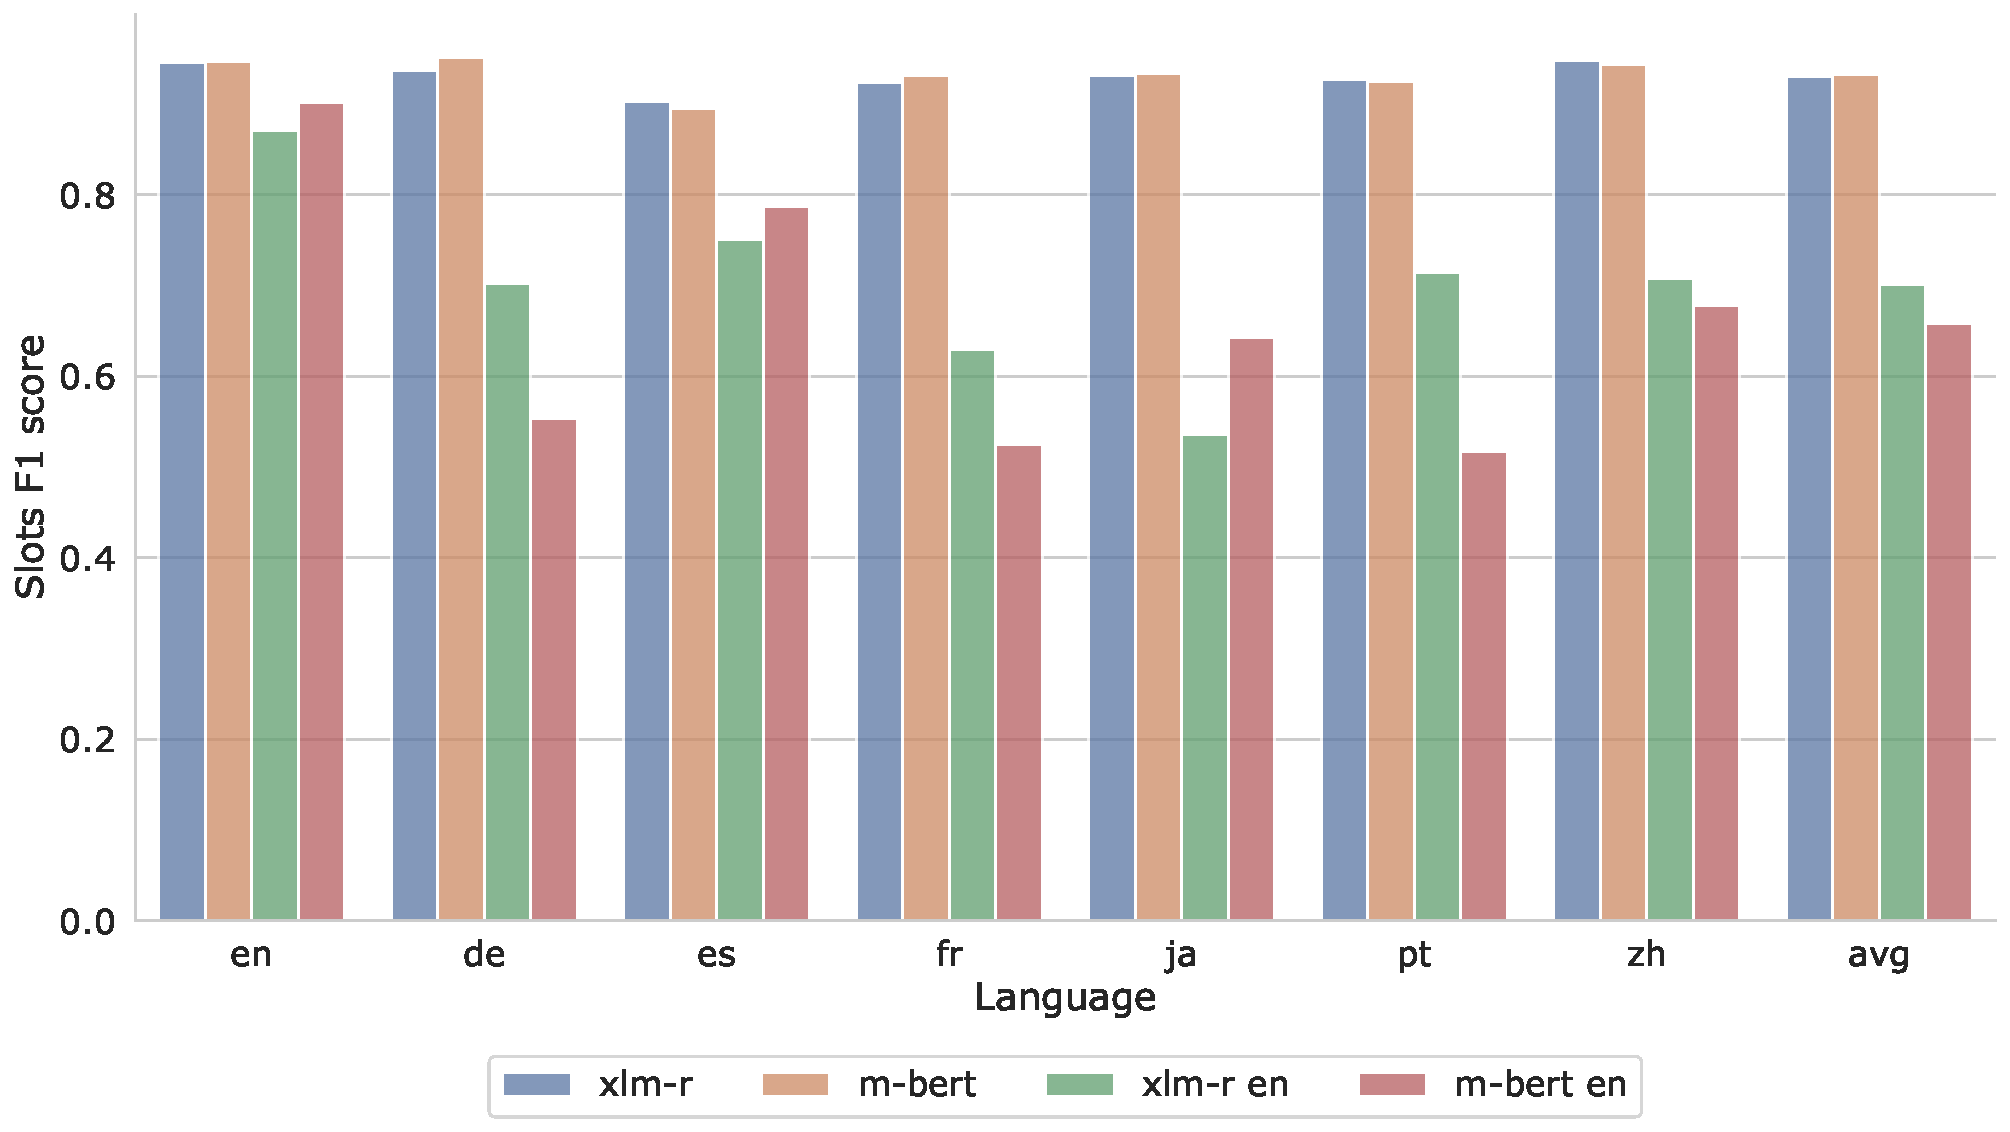
\includegraphics[width=\textwidth]{images/1}
    \caption{Сравнение моделей между собой \textbf{на тестовой выборке} датасета MultiAtis++ по метрике \textbf{Slots F1 score}.}\label{fig:figure1}
\end{figure}
\begin{figure}[H]
    \centering
    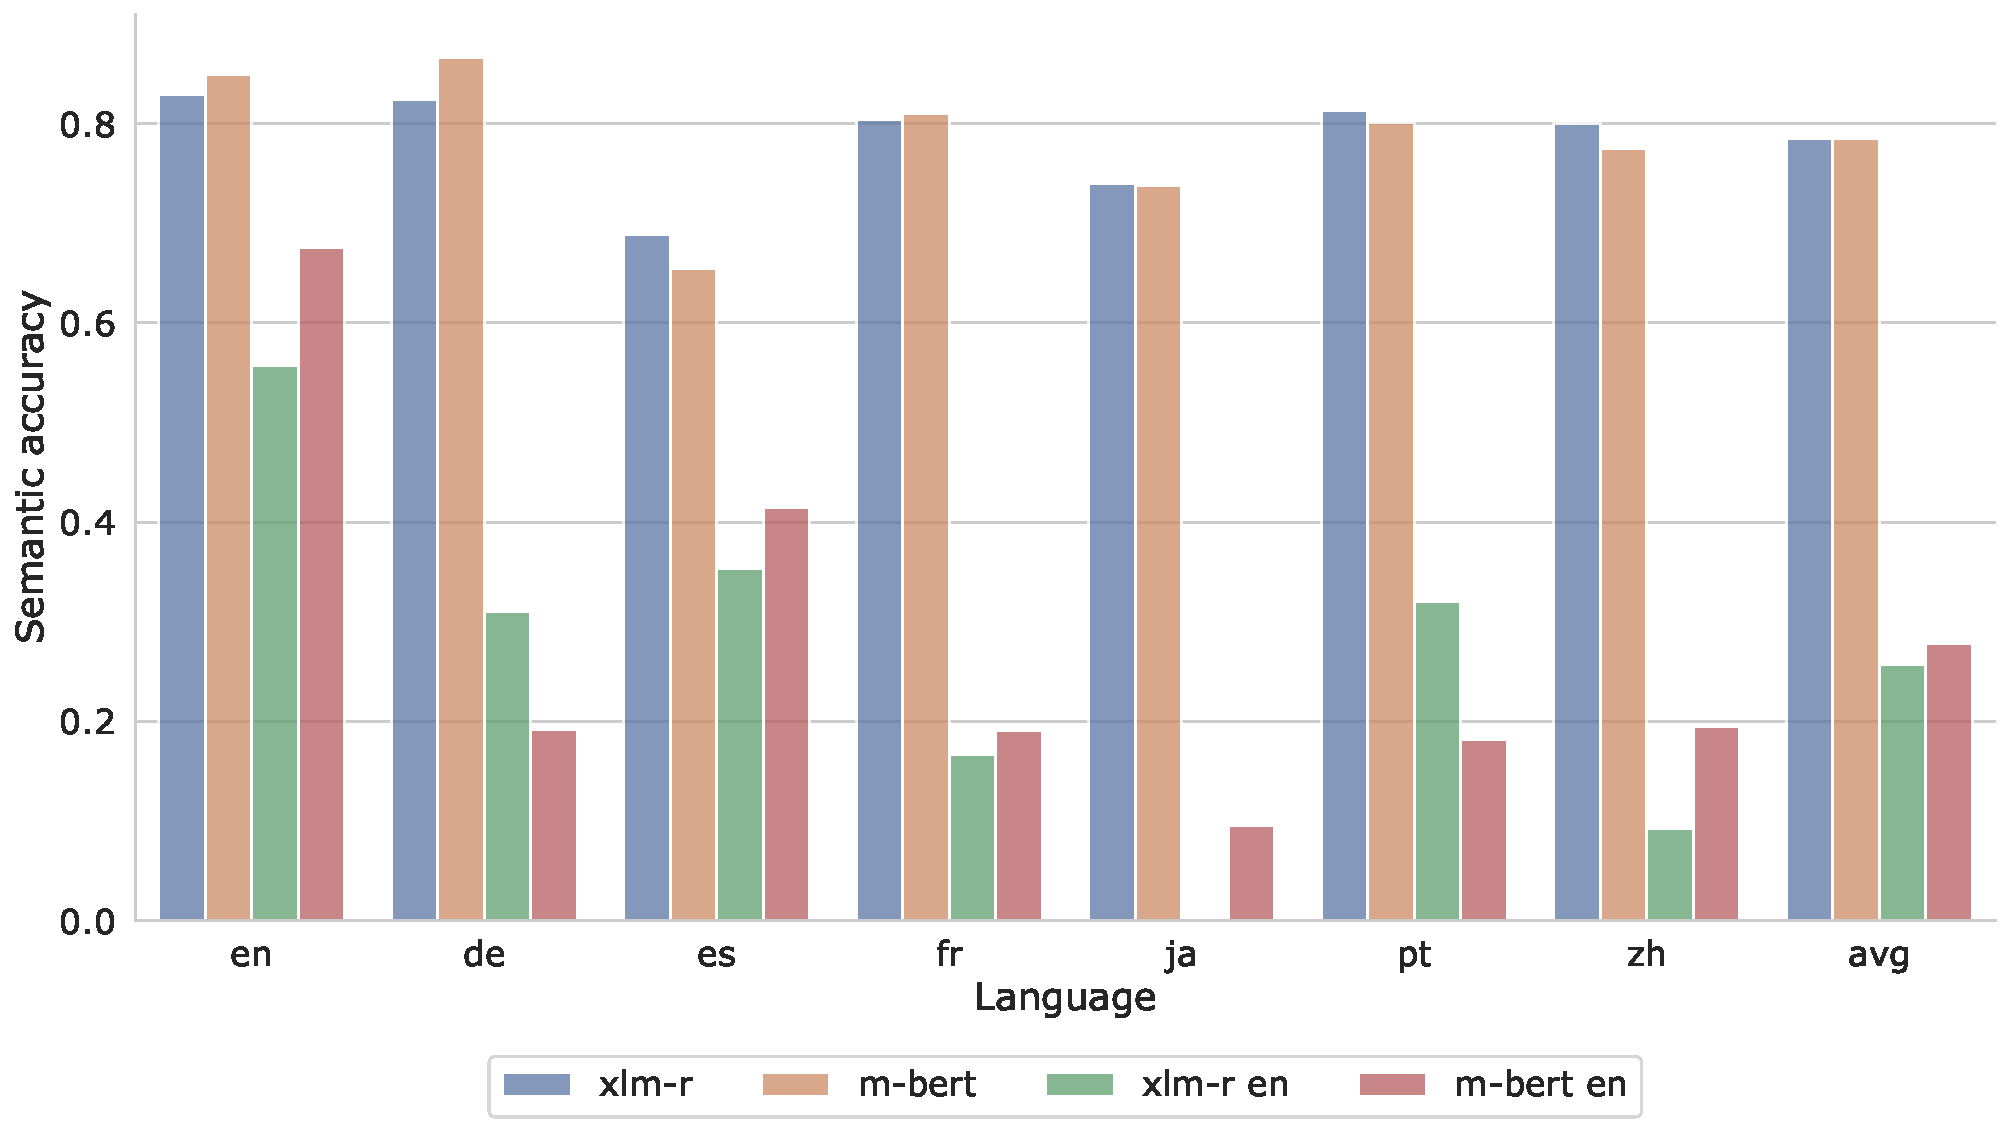
\includegraphics[width=\textwidth]{images/2}
    \caption{Сравнение моделей между собой \textbf{на тестовой выборке} датасета MultiAtis++ по метрике \textbf{Semantic accuracy}.}\label{fig:figure2}
\end{figure}

\begin{figure}[H]
    \centering
    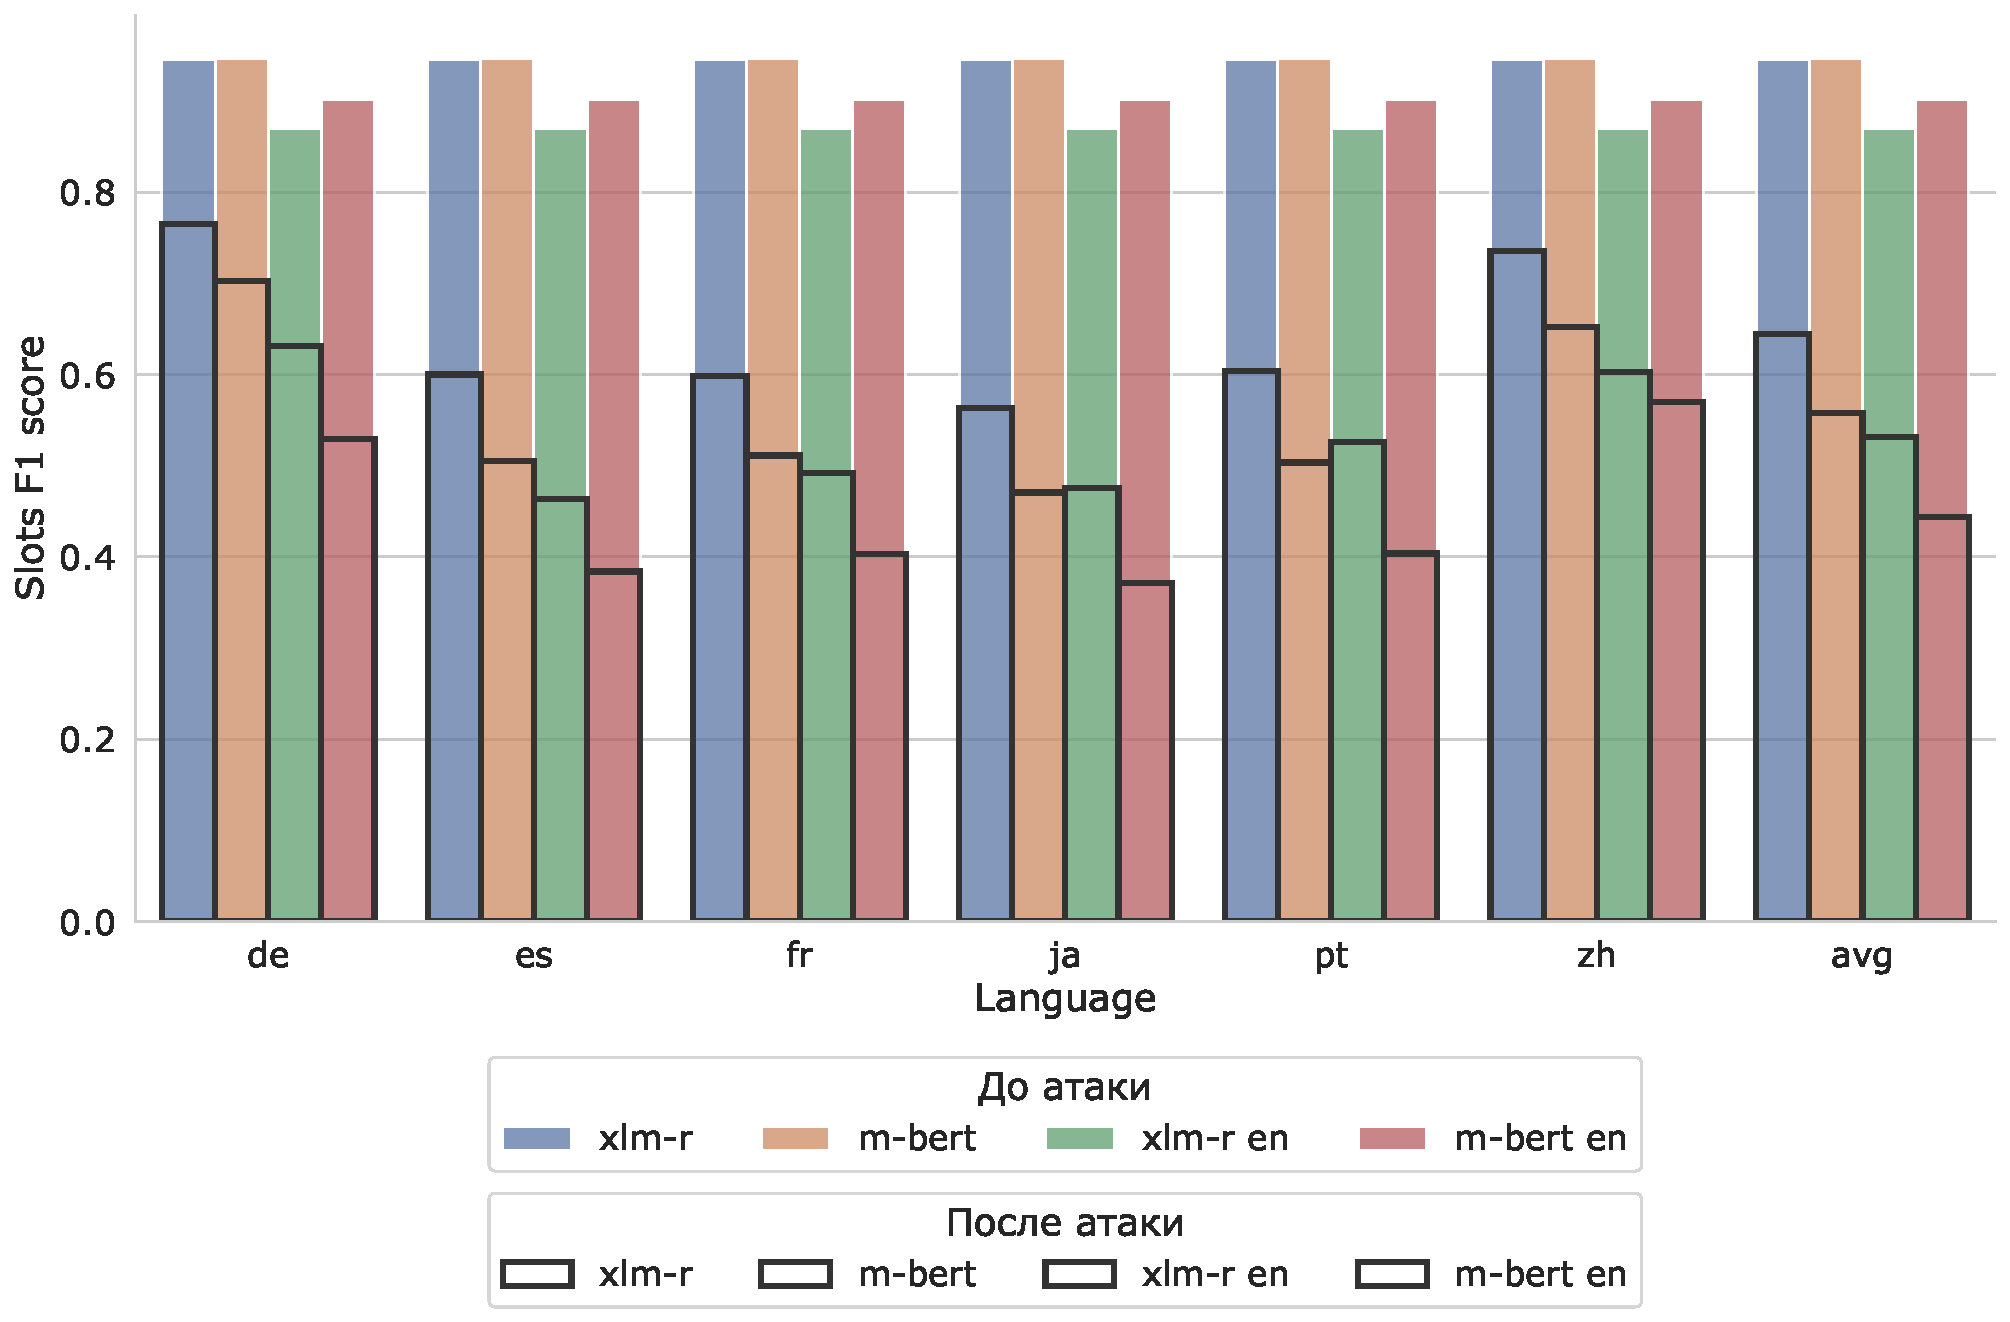
\includegraphics[width=\textwidth]{images/4}
    \caption{Сравнение моделей между собой после \textbf{word-level} атаки на тестовую выборку датасета MultiAtis++ по метрике \textbf{Slots F1 score}.}\label{fig:figure4}
\end{figure}
\begin{figure}[H]
    \centering
    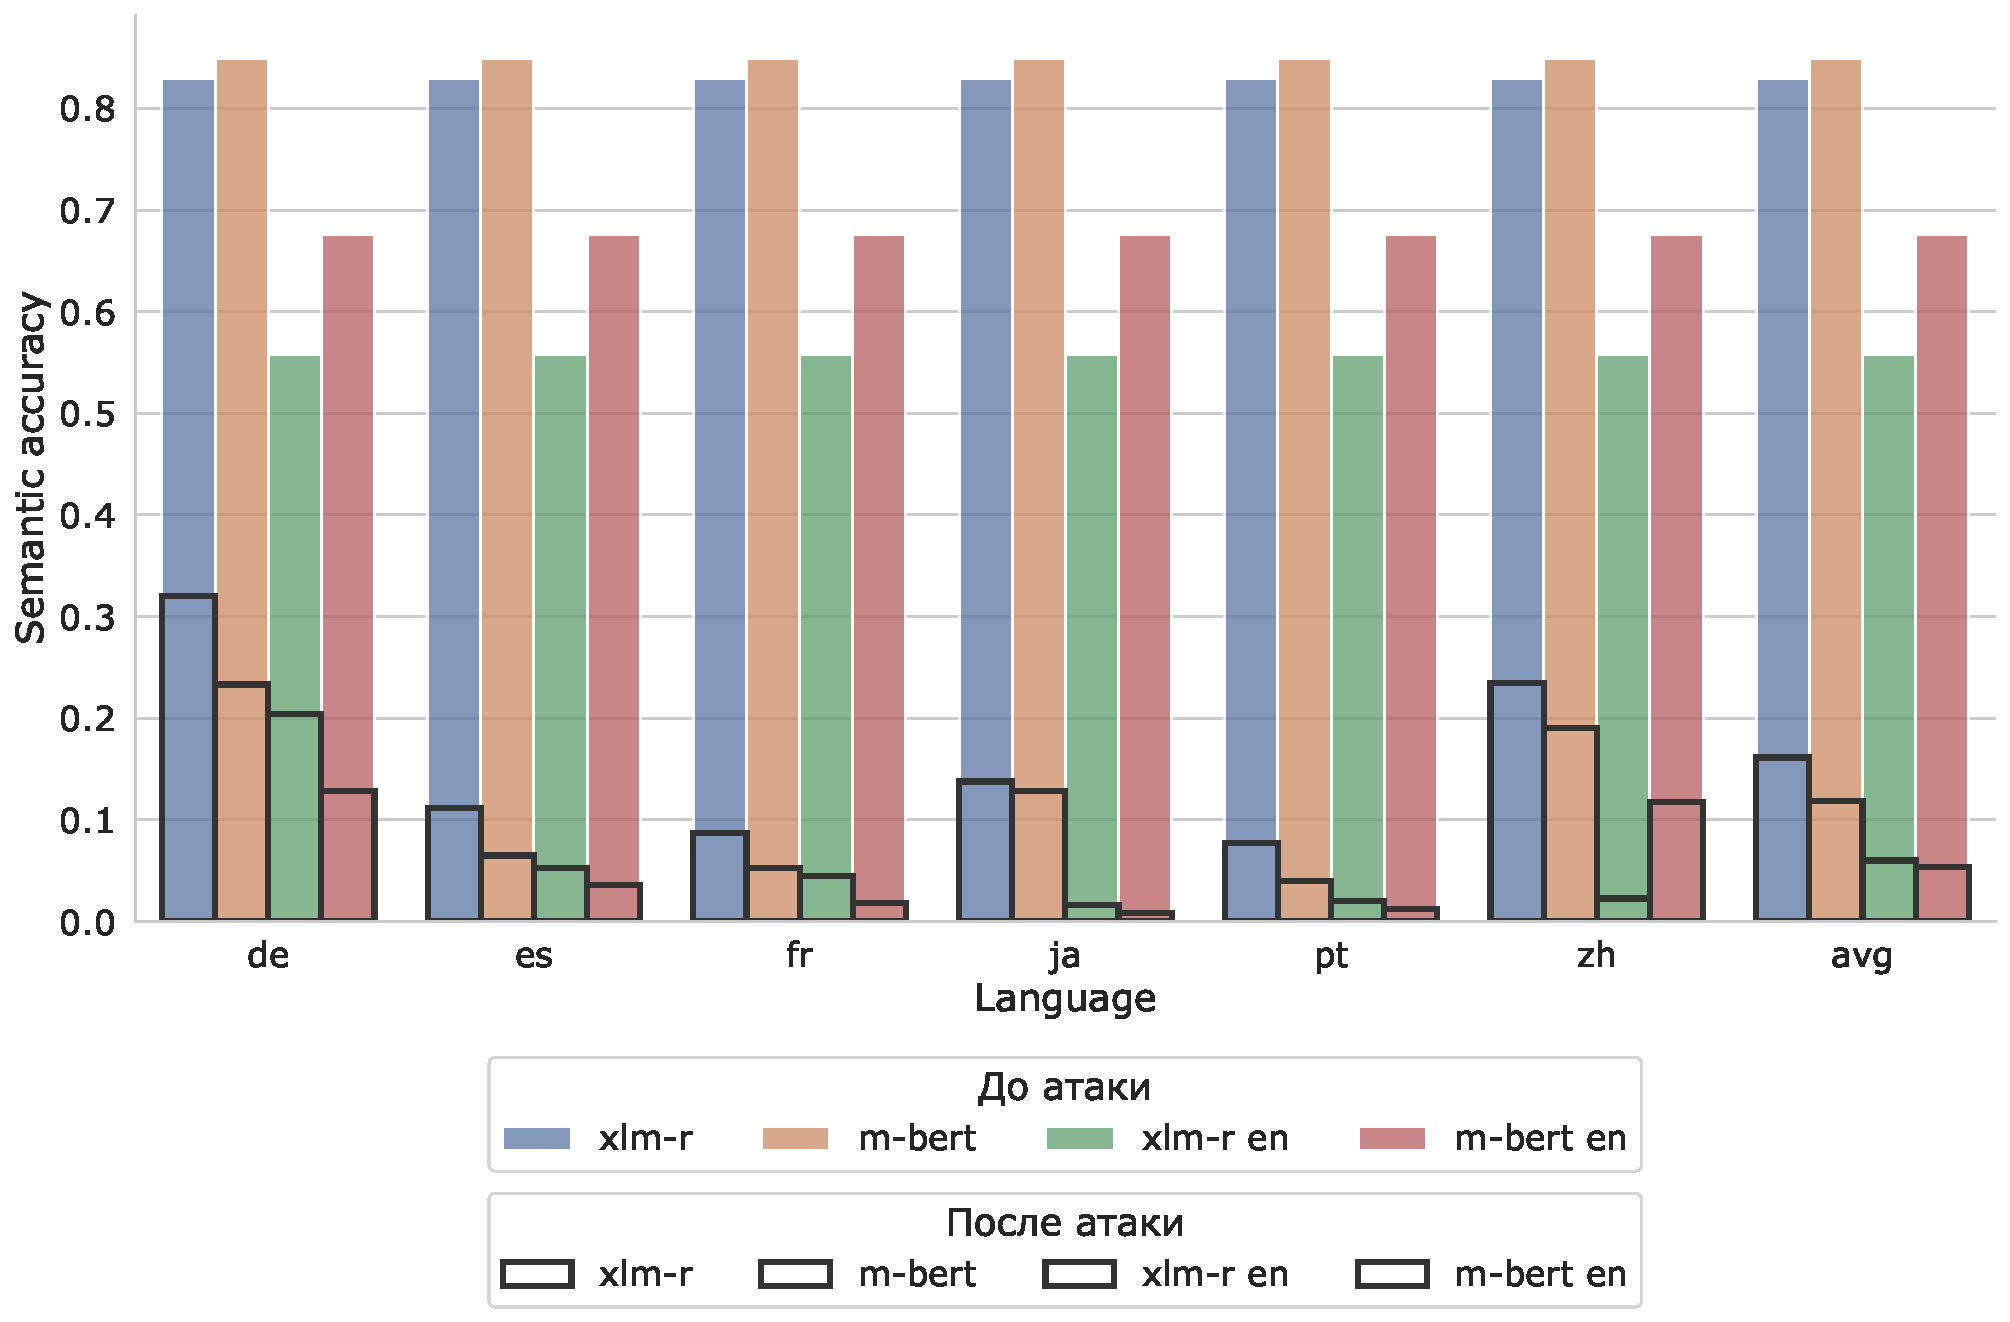
\includegraphics[width=\textwidth]{images/5}
    \caption{Сравнение моделей между собой после \textbf{word-level} атаки на тестовую выборку датасета MultiAtis++ по метрике \textbf{Semantic accuracy}.}\label{fig:figure5}
\end{figure}

\begin{figure}[H]
    \centering
    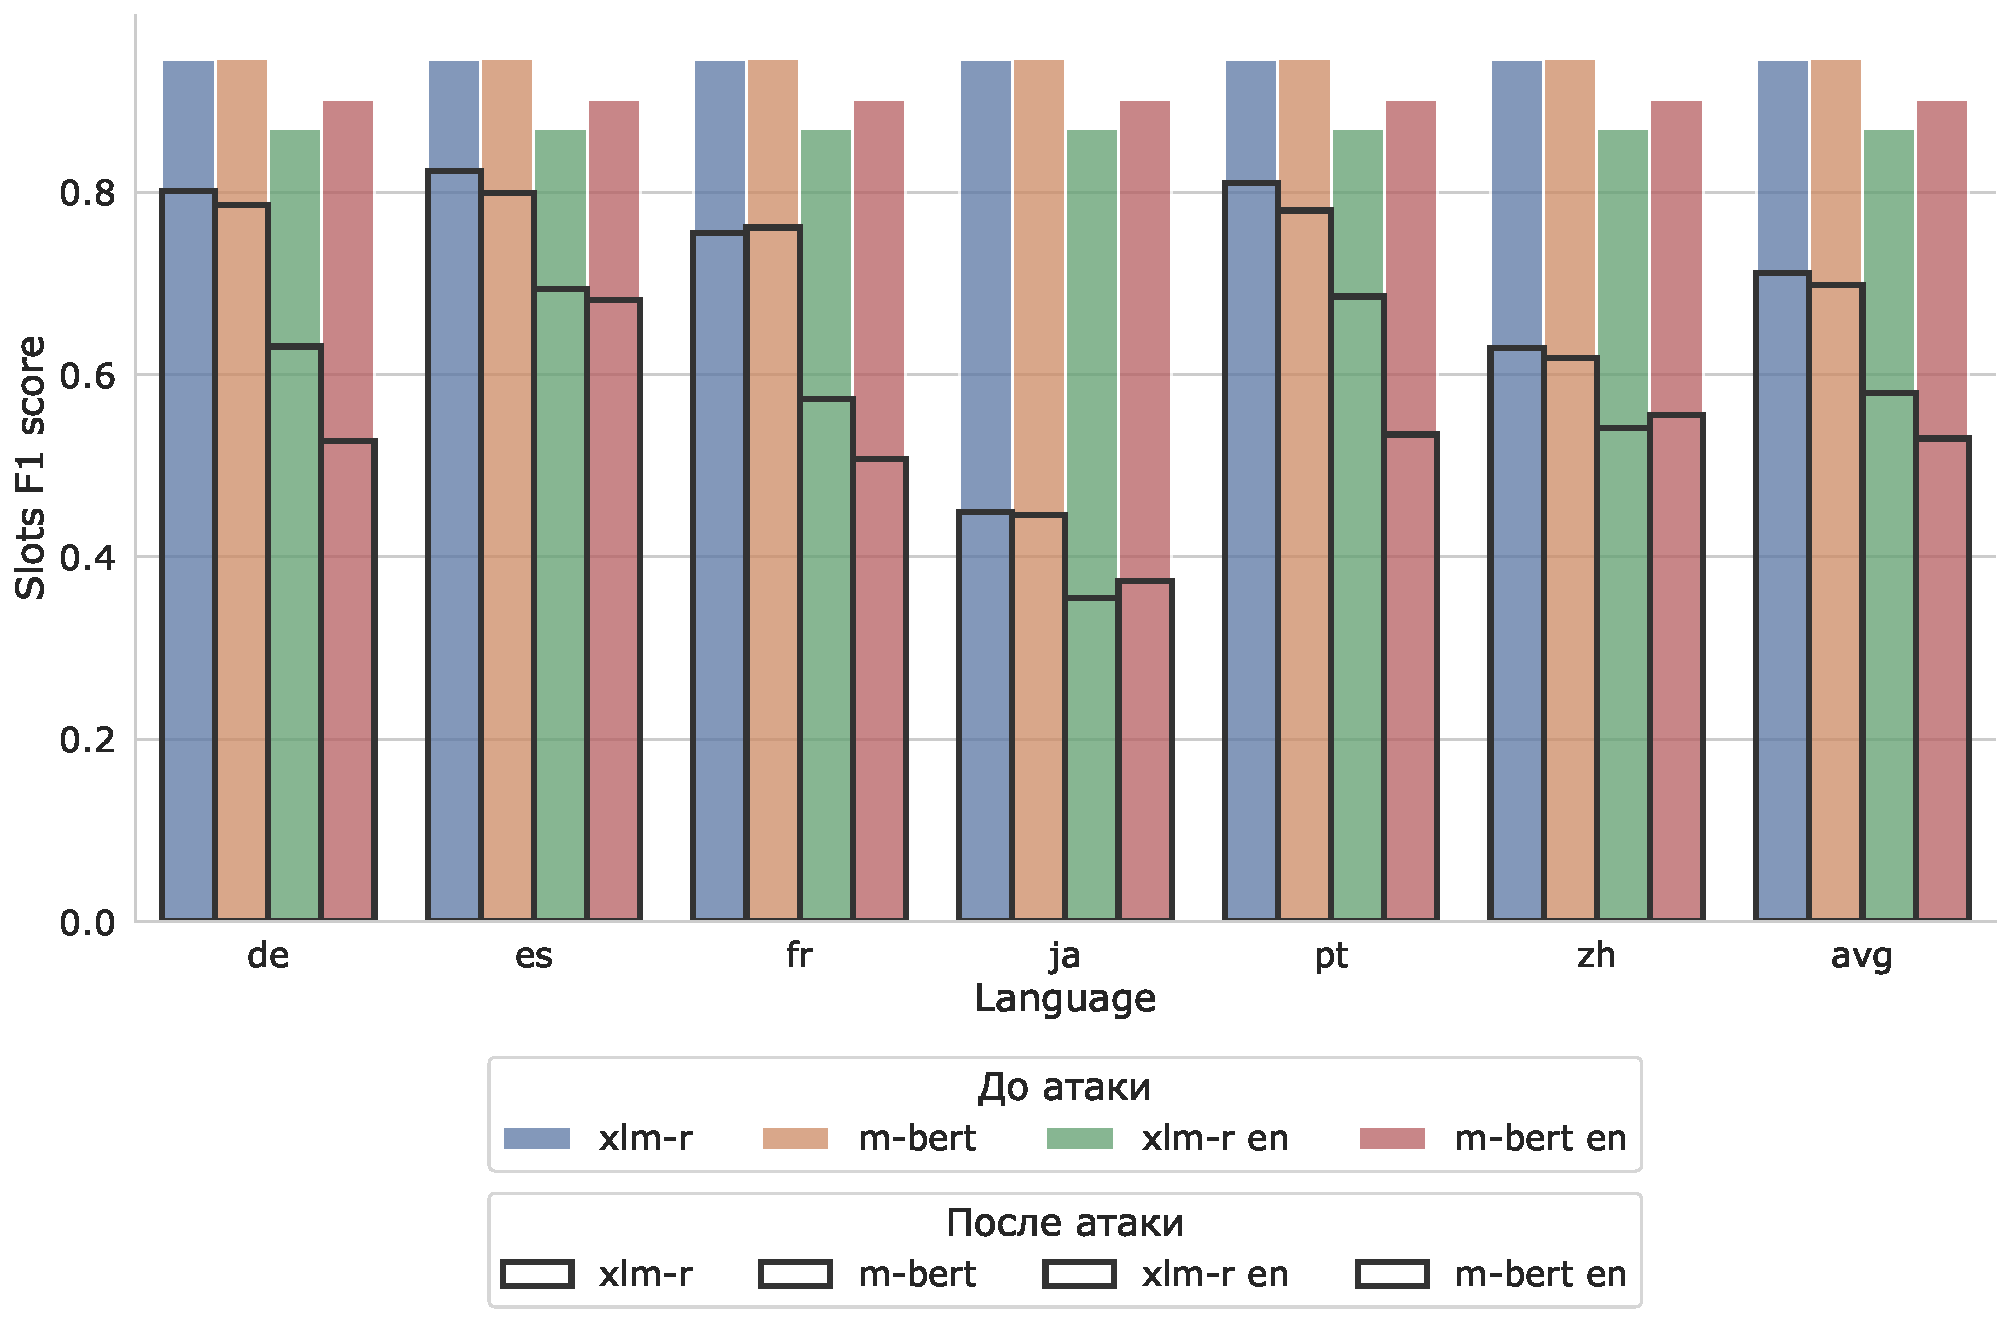
\includegraphics[width=\textwidth]{images/7}
    \caption{Сравнение моделей между собой после \textbf{phrase-level} атаки на тестовую выборку датасета MultiAtis++ по метрике \textbf{Slots F1 score}.}\label{fig:figure7}
\end{figure}
\begin{figure}[H]
    \centering
    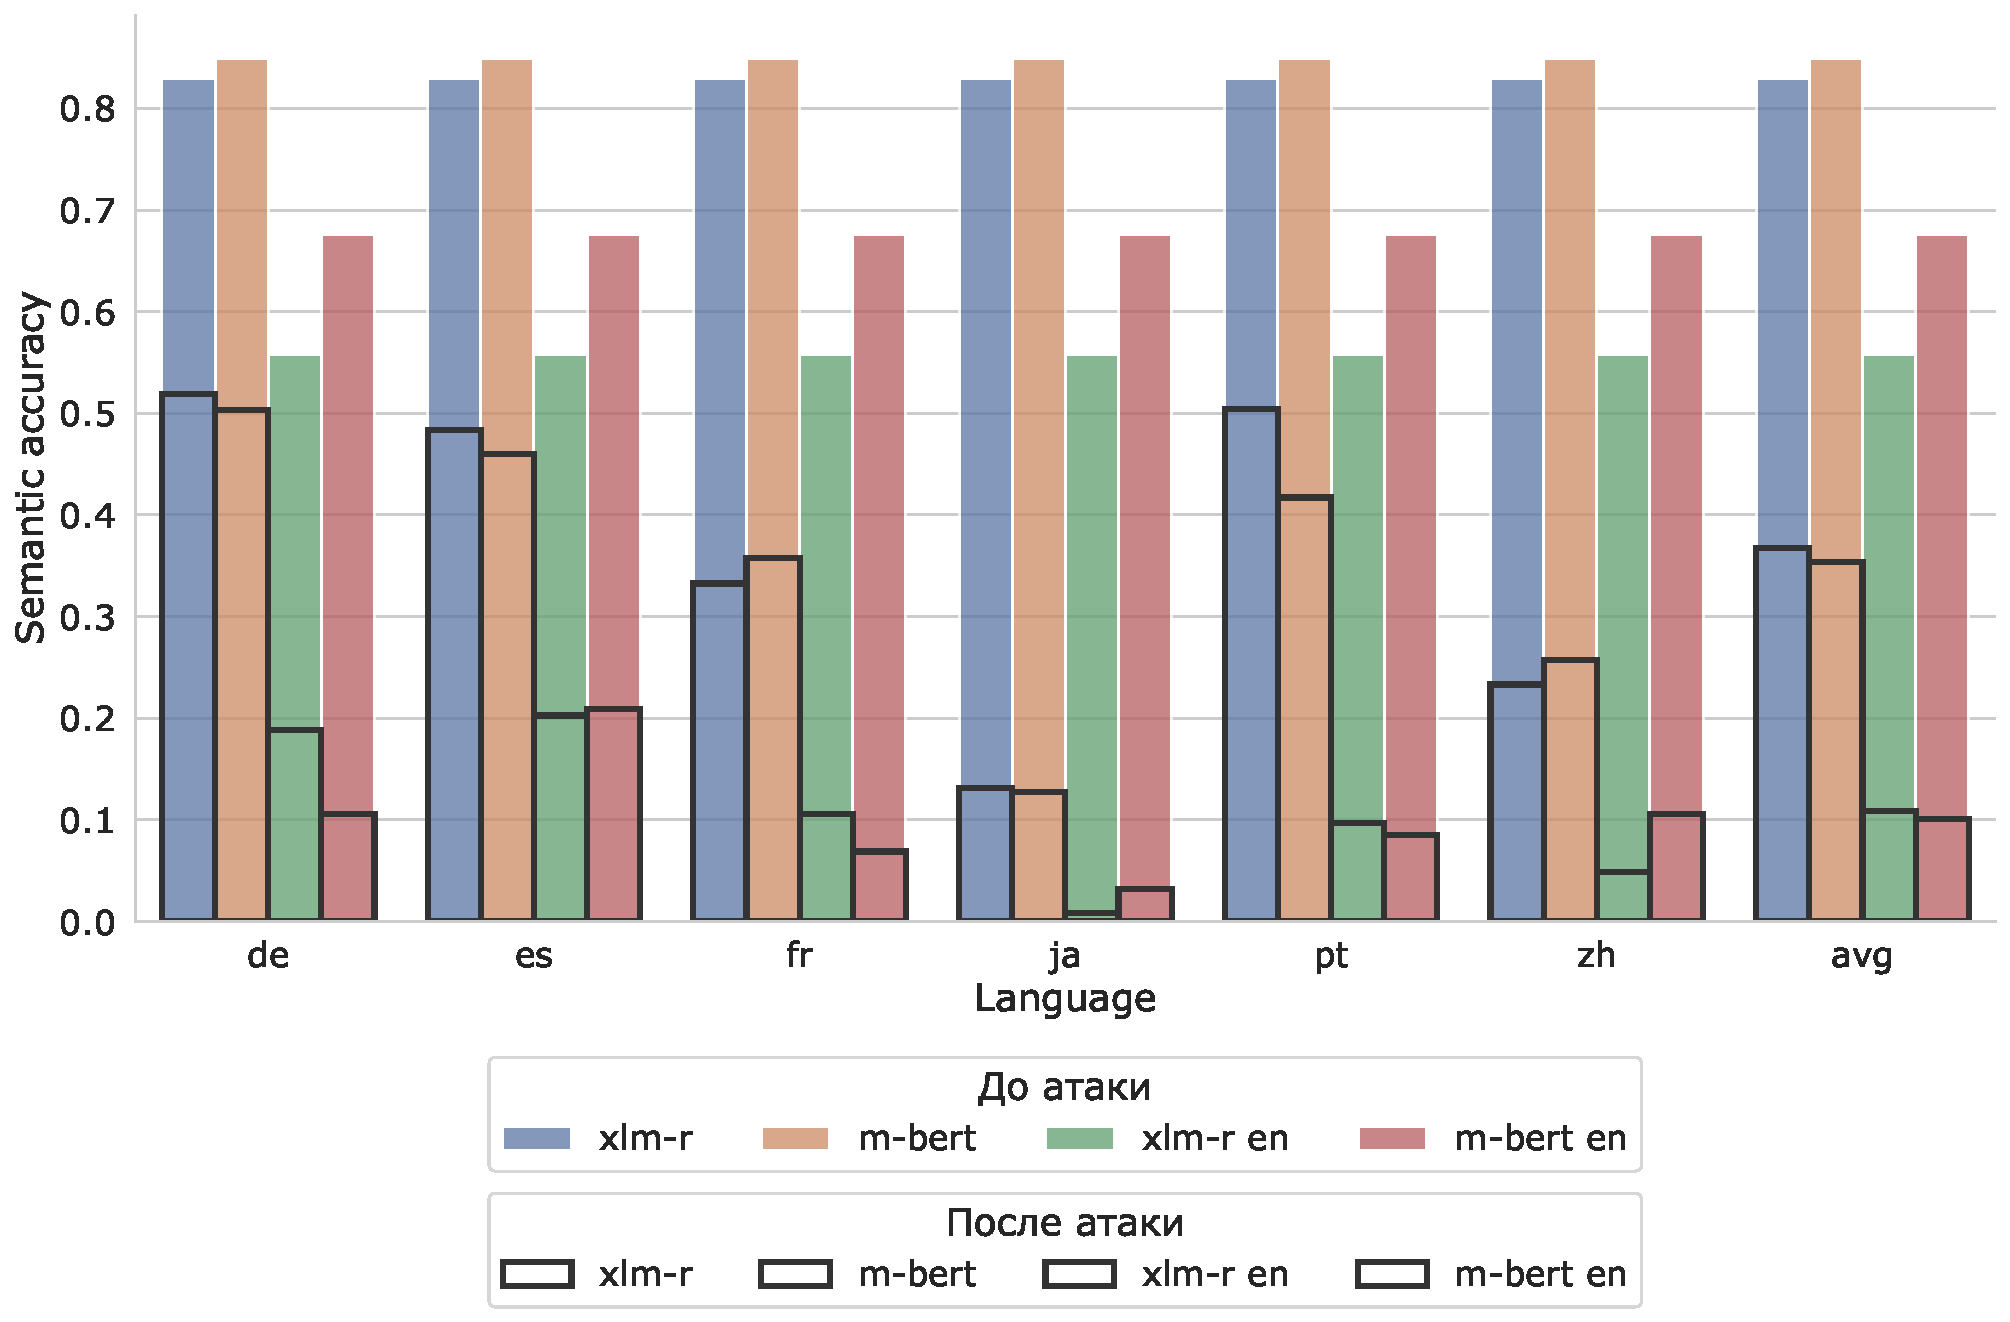
\includegraphics[width=\textwidth]{images/8}
    \caption{Сравнение моделей между собой после \textbf{phrase-level} атаки на тестовую выборку датасета MultiAtis++ по метрике \textbf{Semantic accuracy}.}\label{fig:figure8}
\end{figure}

\begin{figure}[H]
    \centering
    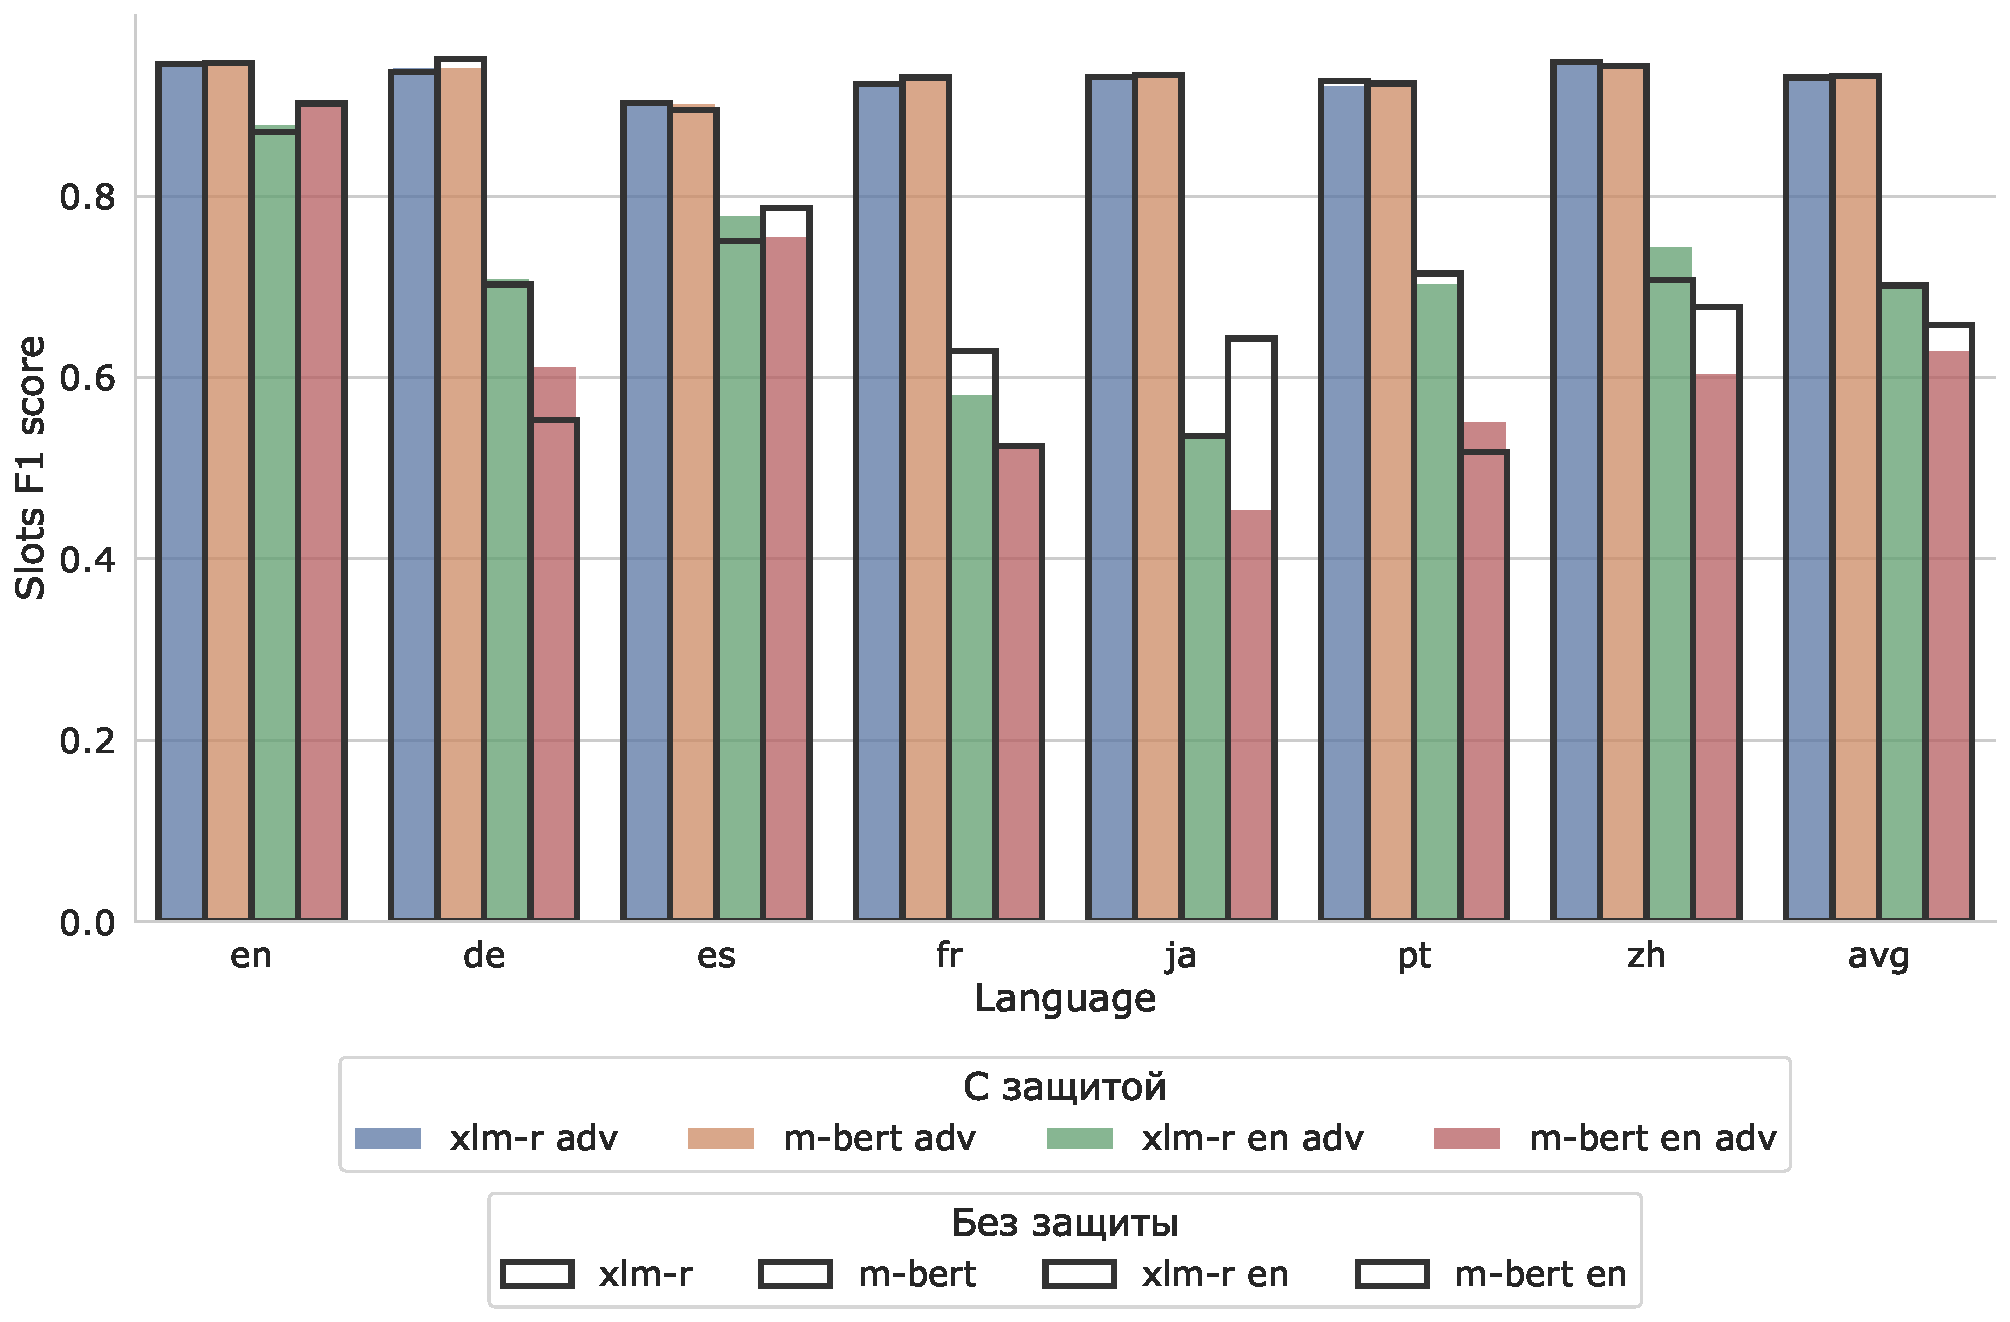
\includegraphics[width=\textwidth]{images/10}
    \caption{Сравнение моделей \textbf{с защитой} между собой \textbf{на тестовой выборке} датасета MultiAtis++ по метрике \textbf{Slots F1 score}.}\label{fig:figure10}
\end{figure}
\begin{figure}[H]
    \centering
    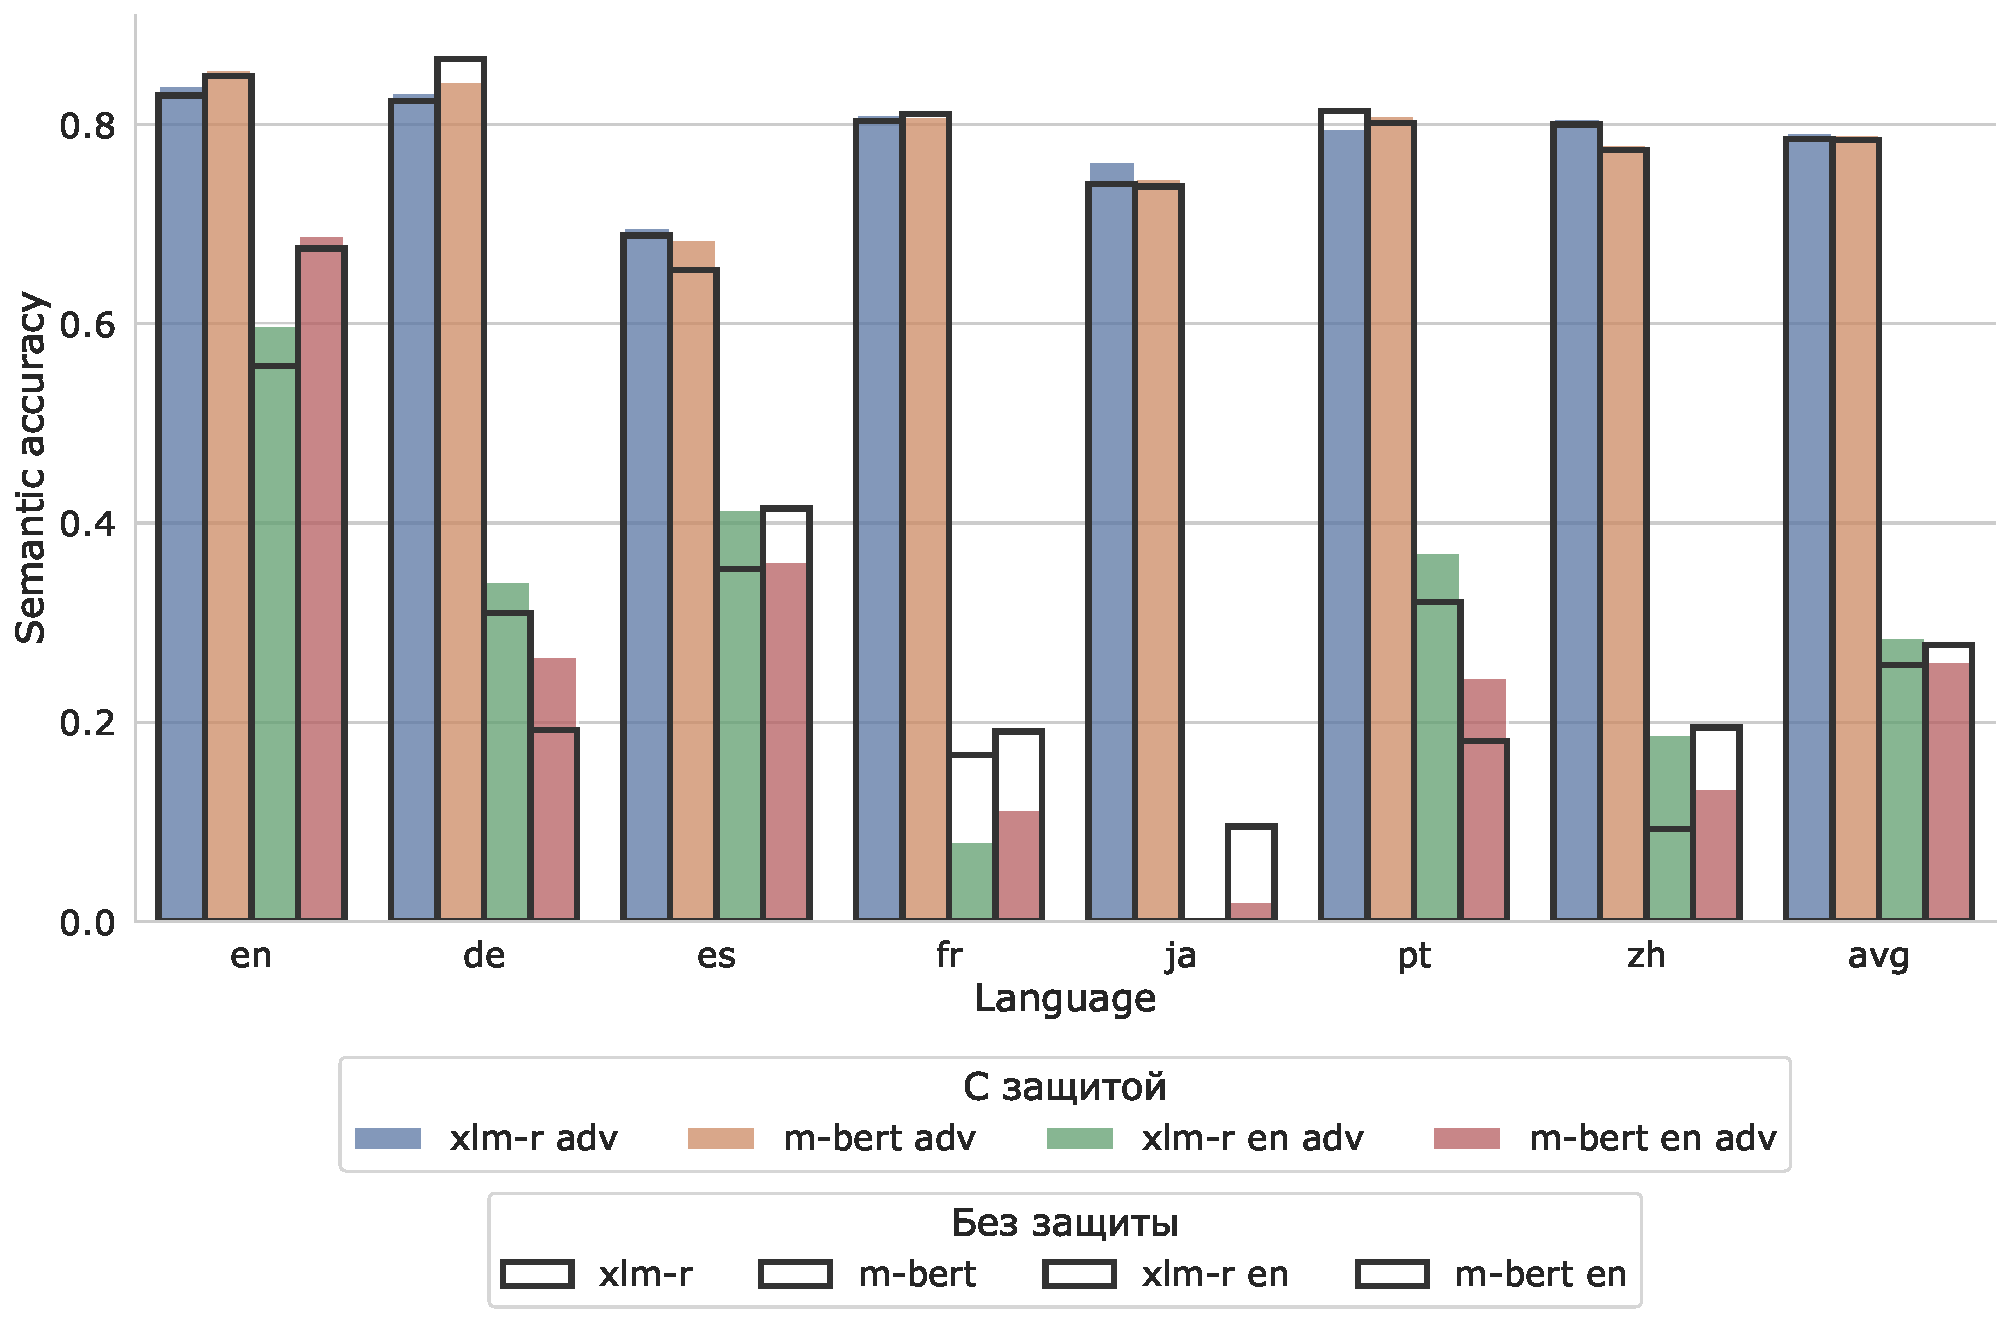
\includegraphics[width=\textwidth]{images/11}
    \caption{Сравнение моделей \textbf{с защитой} между собой \textbf{на тестовой выборке} датасета MultiAtis++ по метрике \textbf{Semantic accuracy}.}\label{fig:figure11}
\end{figure}

\begin{figure}[H]
    \centering
    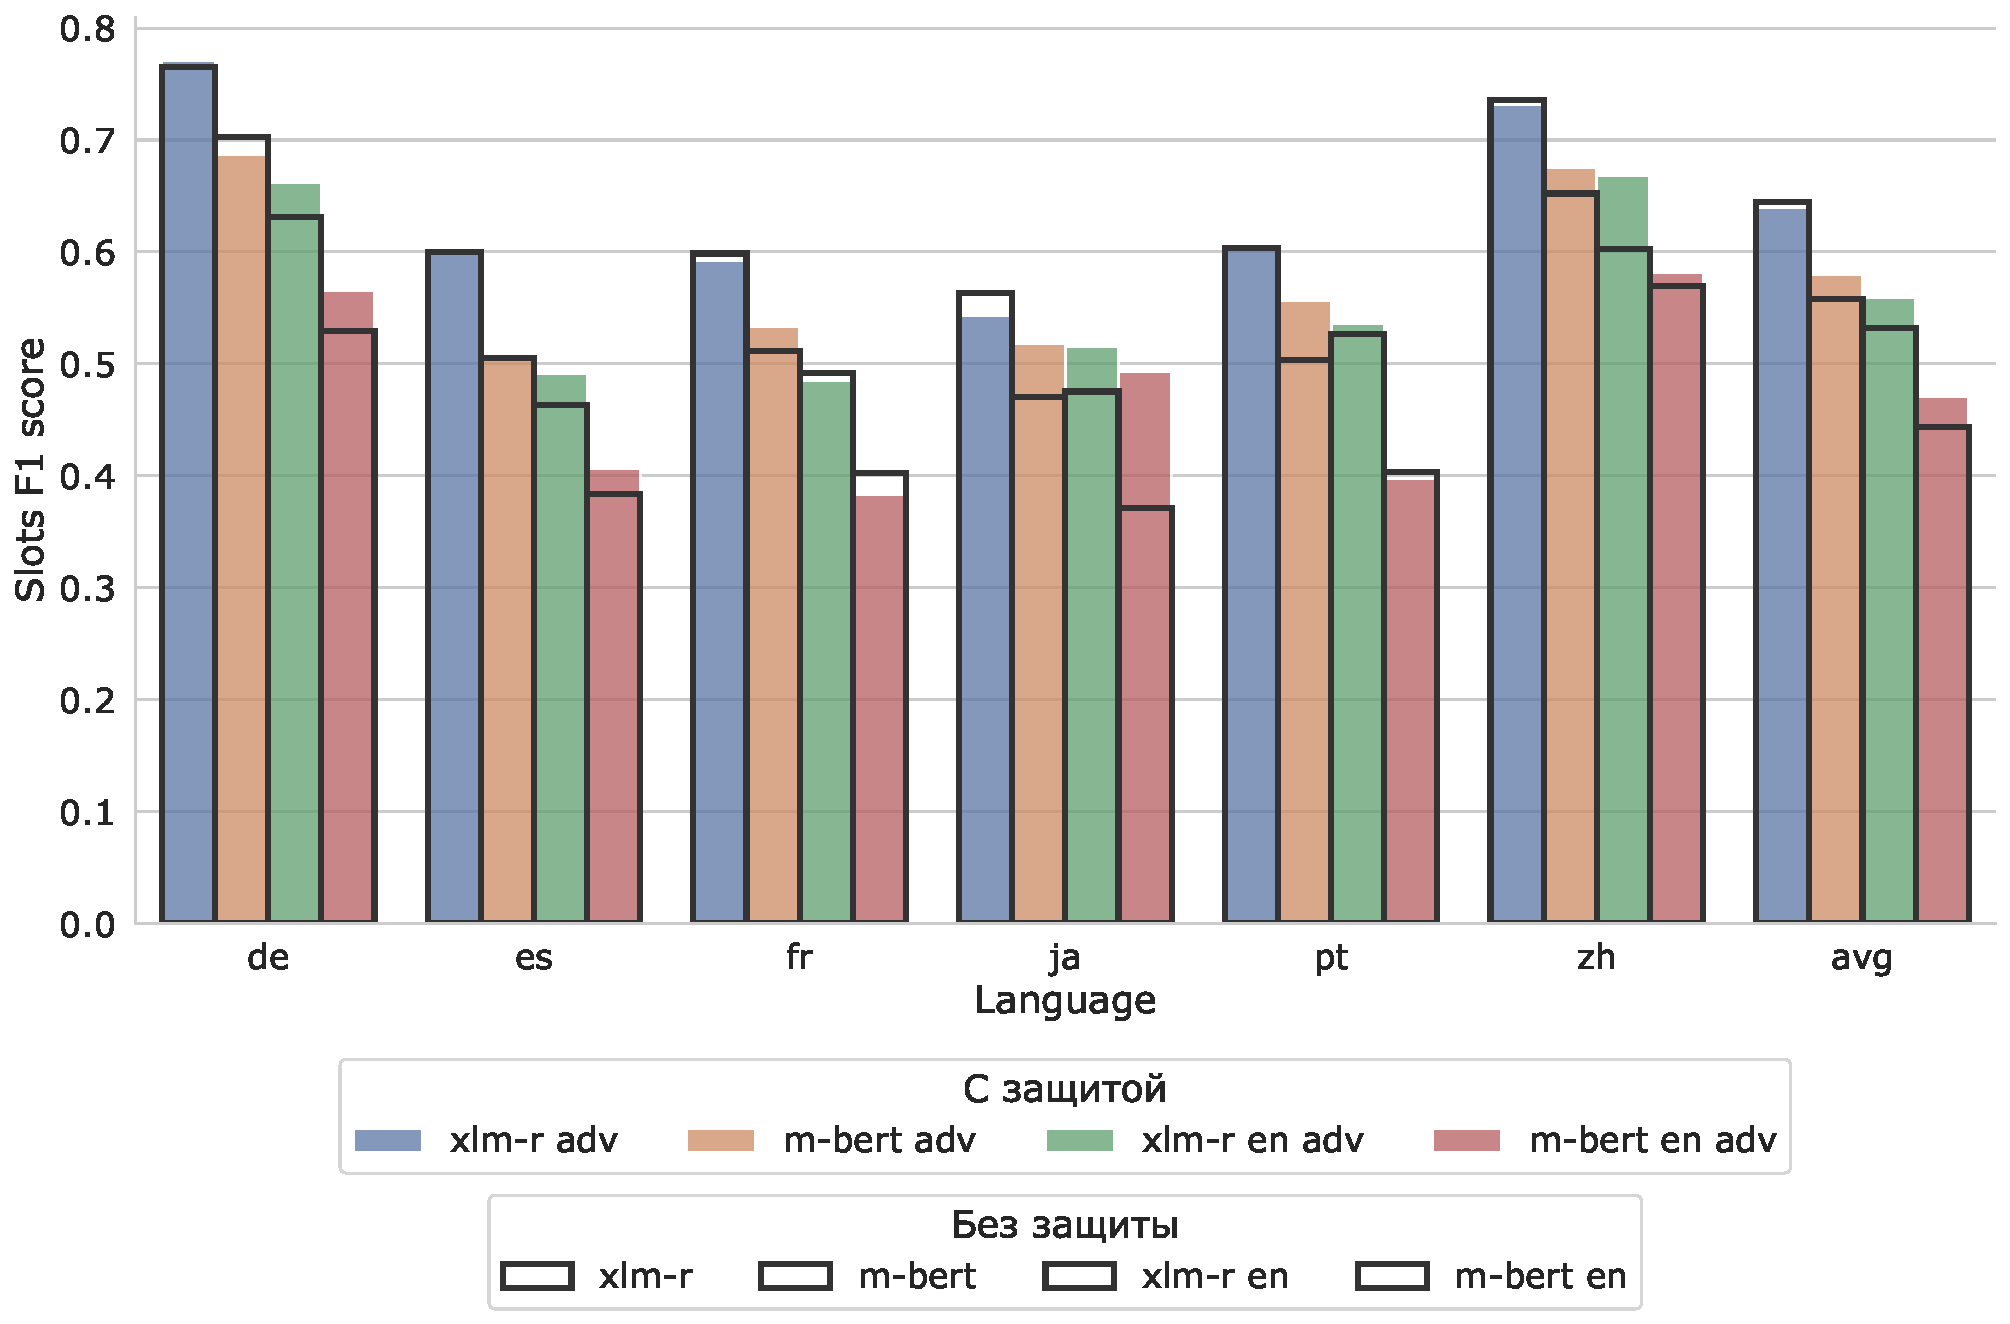
\includegraphics[width=\textwidth]{images/13}
    \caption{Сравнение моделей \textbf{с защитой} между собой после \textbf{word-level} атаки на тестовую выборку датасета MultiAtis++ по метрике \textbf{Slots F1 score}.}\label{fig:figure13}
\end{figure}
\begin{figure}[H]
    \centering
    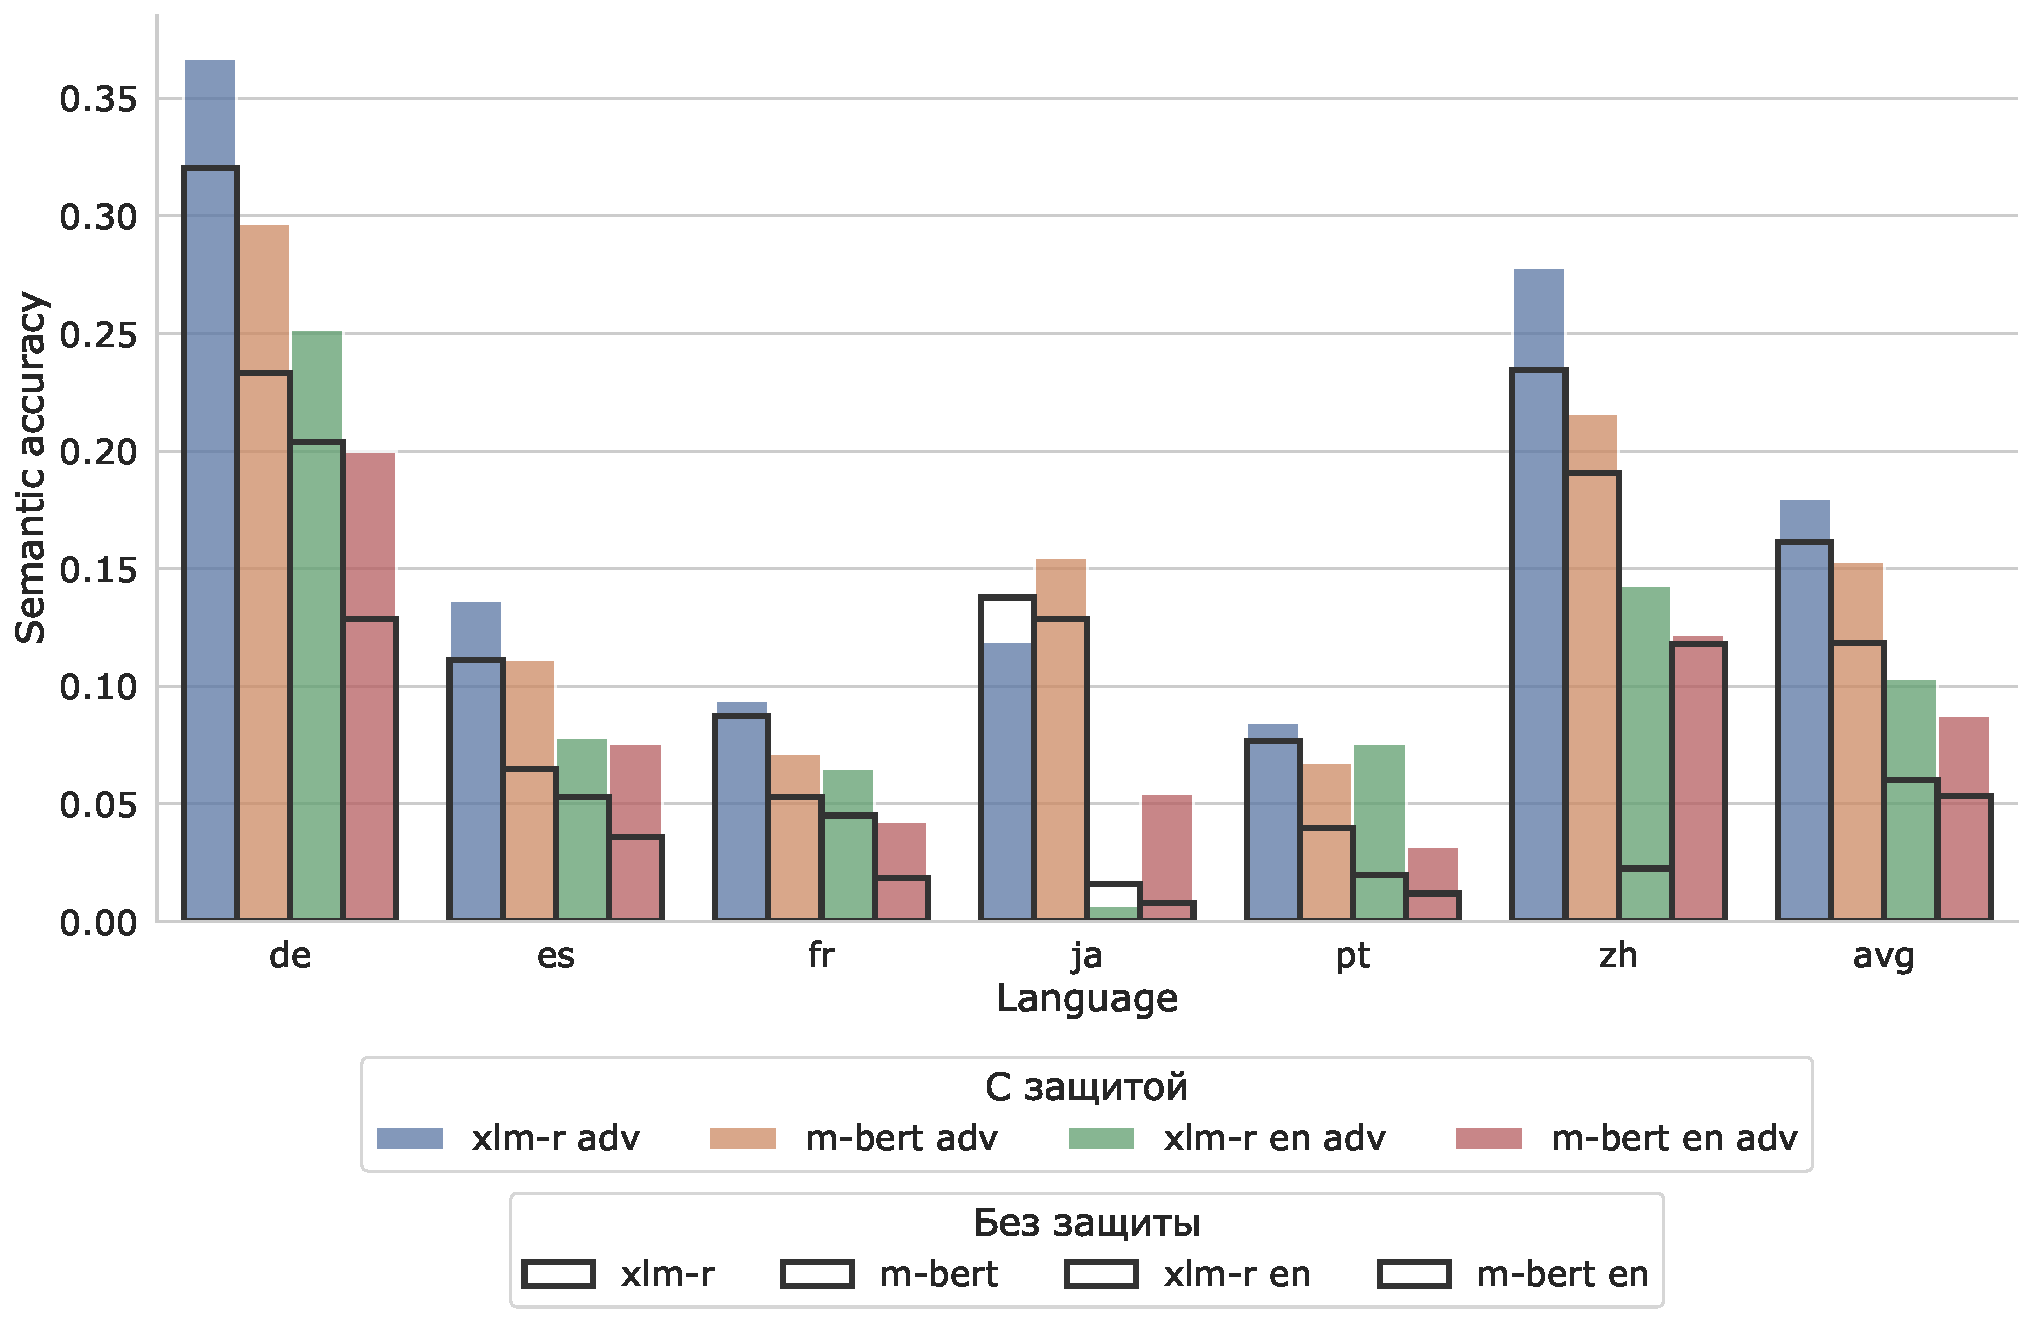
\includegraphics[width=\textwidth]{images/14}
    \caption{Сравнение моделей \textbf{с защитой} между собой после \textbf{word-level} атаки на тестовую выборку датасета MultiAtis++ по метрике \textbf{Semantic accuracy}.}\label{fig:figure14}
\end{figure}

\begin{figure}[H]
    \centering
    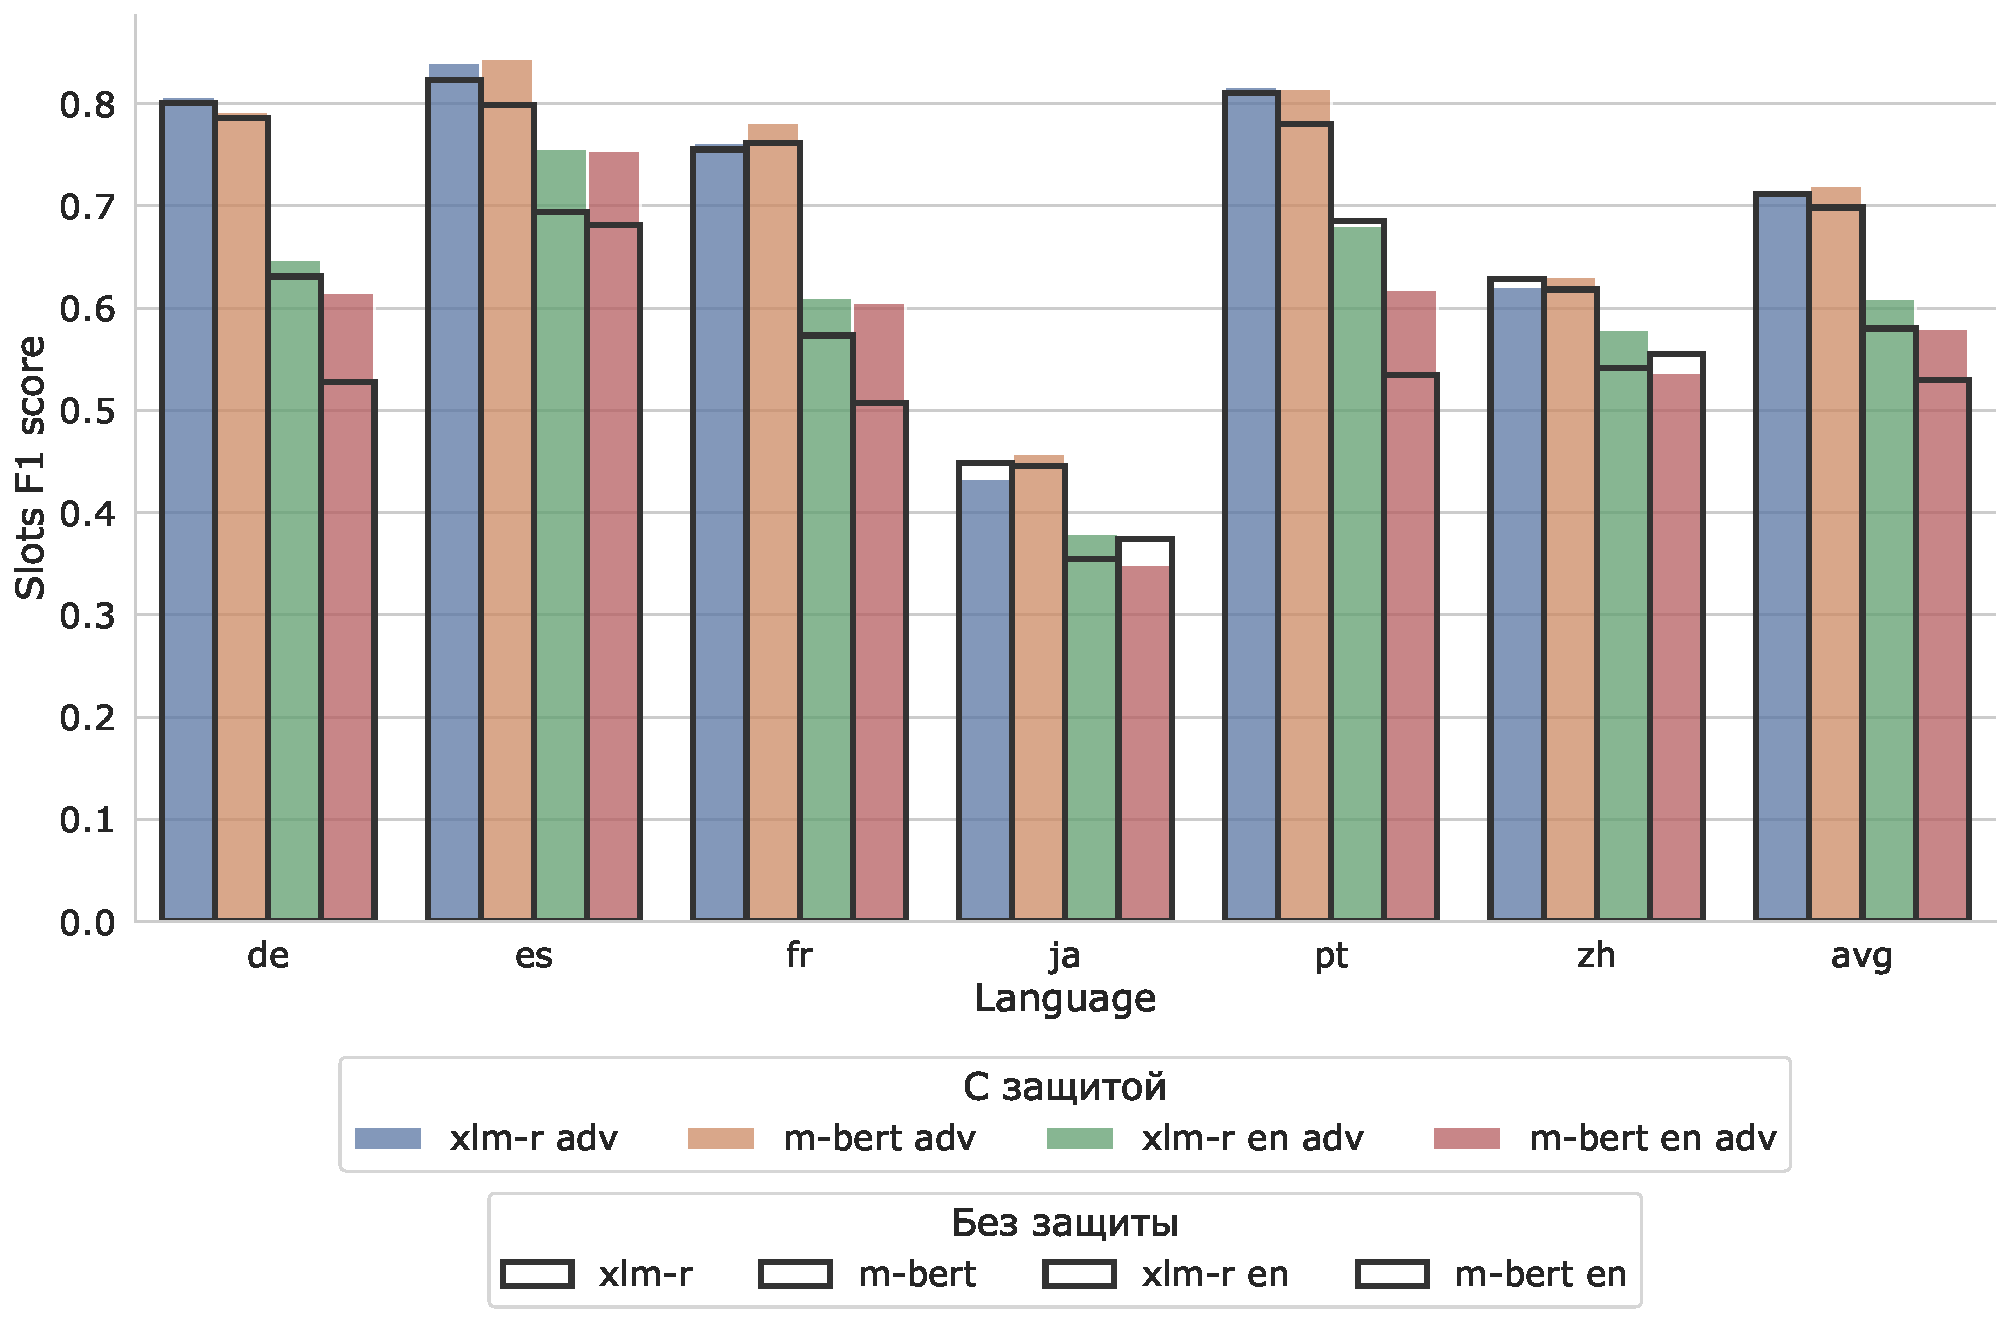
\includegraphics[width=\textwidth]{images/16}
    \caption{Сравнение моделей \textbf{с защитой} между собой после \textbf{phrase-level} атаки на тестовую выборку датасета MultiAtis++ по метрике \textbf{Slots F1 score}.}\label{fig:figure16}
\end{figure}
\begin{figure}[H]
    \centering
    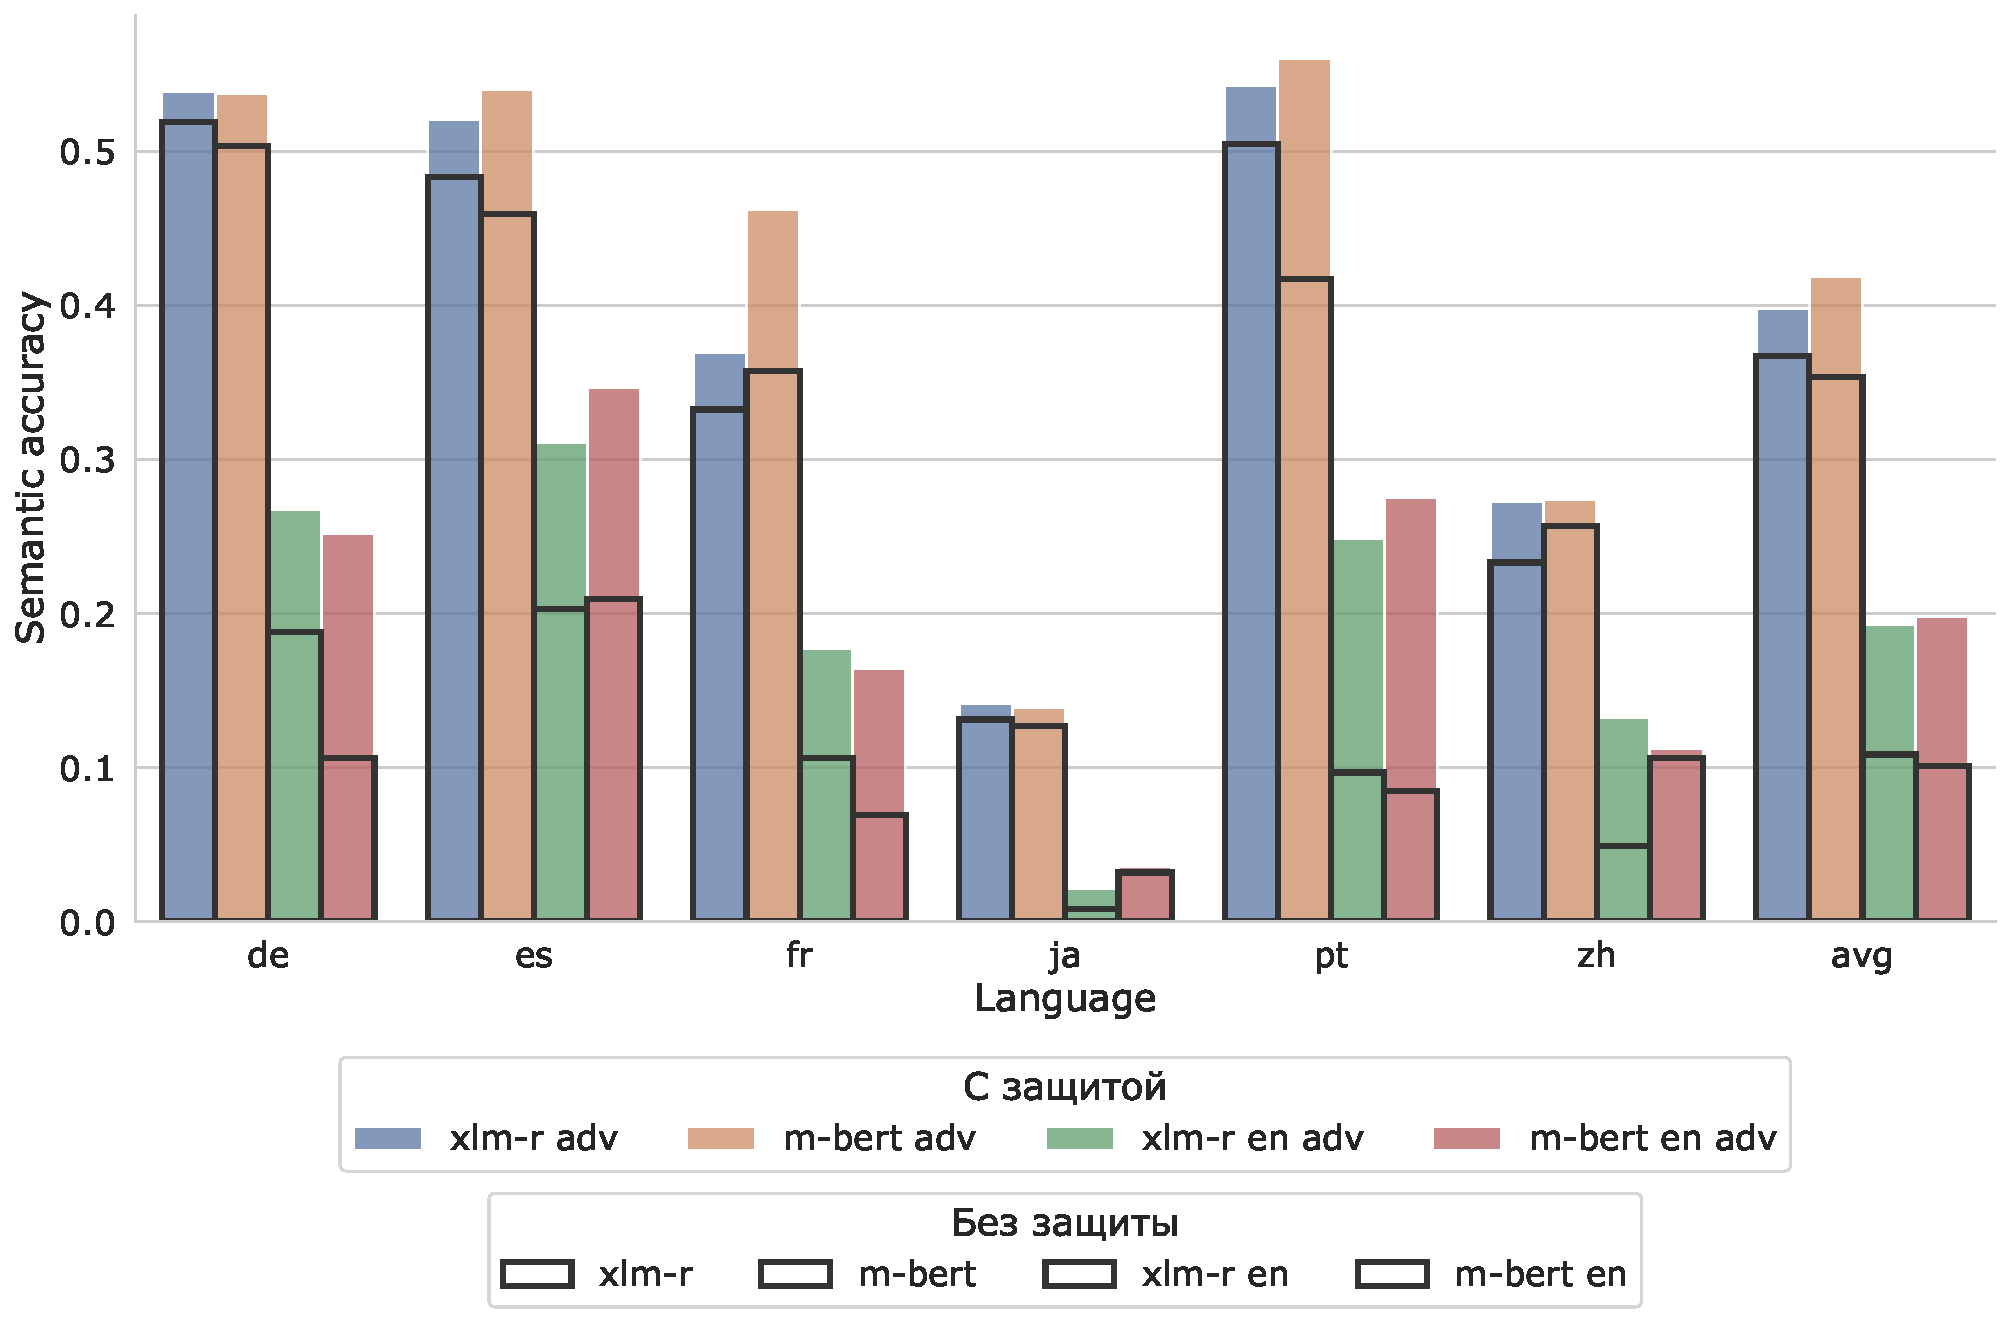
\includegraphics[width=\textwidth]{images/17}
    \caption{Сравнение моделей \textbf{с защитой} между собой после \textbf{phrase-level} атаки на тестовую выборку датасета MultiAtis++ по метрике \textbf{Semantic accuracy}.}\label{fig:figure17}
\end{figure}

\newpage

\subsection{Таблицы с результатами экспериментов}\label{subsec:tables}

\begin{table}[H]
	\resizebox{\textwidth}{!}{
		\begin{tabular}{|>{\bfseries}l|c|c|c|c|c|c|c|c|}
			\hline
			& en & de & es & fr & ja & pt & zh & avg \\ \hline
			xlm-r&$0.980$ & $0.975$ & $0.968$ & $0.972$ & $0.977$ & $0.970$ & $0.968$ & $0.973$ \\ \hline
			m-bert&$0.977$ & $0.977$ & $0.963$ & $0.966$ & $0.959$ & $0.967$ & $0.962$ & $0.967$ \\ \hline
			xlm-r en&$0.903$ & $0.885$ & $0.882$ & $0.879$ & $0.830$ & $0.846$ & $0.856$ & $0.869$ \\ \hline
			m-bert en&$0.951$ & $0.828$ & $0.865$ & $0.877$ & $0.750$ & $0.853$ & $0.795$ & $0.845$ \\ \hline
		\end{tabular}
	}\caption{Сравнение моделей между собой \textbf{на тестовой выборке} датасета MultiAtis++ по метрике \textbf{Intent accuracy}. По колонкам языки тестовых подвыборок, по рядам тестируемые модели.}\label{tab:table0}
\end{table}
\begin{table}[H]
	\resizebox{\textwidth}{!}{
		\begin{tabular}{|>{\bfseries}l|c|c|c|c|c|c|c|c|}
			\hline
			& en & de & es & fr & ja & pt & zh & avg \\ \hline
			xlm-r&$0.945$ & $0.937$ & $0.902$ & $0.924$ & $0.931$ & $0.927$ & $0.948$ & $0.931$ \\ \hline
			m-bert&$0.947$ & $0.951$ & $0.895$ & $0.931$ & $0.933$ & $0.924$ & $0.944$ & $0.932$ \\ \hline
			xlm-r en&$0.871$ & $0.702$ & $0.750$ & $0.629$ & $0.535$ & $0.715$ & $0.707$ & $0.701$ \\ \hline
			m-bert en&$0.902$ & $0.553$ & $0.787$ & $0.524$ & $0.643$ & $0.517$ & $0.678$ & $0.658$ \\ \hline
		\end{tabular}
	}\caption{Сравнение моделей между собой \textbf{на тестовой выборке} датасета MultiAtis++ по метрике \textbf{Slots F1 score}. По колонкам языки тестовых подвыборок, по рядам тестируемые модели.}\label{tab:table1}
\end{table}
\begin{table}[H]
	\resizebox{\textwidth}{!}{
		\begin{tabular}{|>{\bfseries}l|c|c|c|c|c|c|c|c|}
			\hline
			& en & de & es & fr & ja & pt & zh & avg \\ \hline
			xlm-r&$0.829$ & $0.824$ & $0.689$ & $0.804$ & $0.740$ & $0.813$ & $0.800$ & $0.786$ \\ \hline
			m-bert&$0.849$ & $0.866$ & $0.654$ & $0.811$ & $0.738$ & $0.801$ & $0.775$ & $0.785$ \\ \hline
			xlm-r en&$0.558$ & $0.310$ & $0.354$ & $0.167$ & $0.000$ & $0.321$ & $0.093$ & $0.257$ \\ \hline
			m-bert en&$0.675$ & $0.192$ & $0.415$ & $0.191$ & $0.095$ & $0.181$ & $0.195$ & $0.278$ \\ \hline
		\end{tabular}
	}\caption{Сравнение моделей между собой \textbf{на тестовой выборке} датасета MultiAtis++ по метрике \textbf{Semantic accuracy}. По колонкам языки тестовых подвыборок, по рядам тестируемые модели.}\label{tab:table2}
\end{table}

\begin{table}[H]
	\resizebox{\textwidth}{!}{
		\begin{tabular}{|>{\bfseries}l|c|c|c|c|c|c|c|}
			\hline
			& de & es & fr & ja & pt & zh & avg \\ \hline
			xlm-r&$0.934$ & $0.881$ & $0.866$ & $0.842$ & $0.894$ & $0.890$ & $0.885$ \\ \hline
			m-bert&$0.902$ & $0.881$ & $0.858$ & $0.868$ & $0.854$ & $0.865$ & $0.871$ \\ \hline
			xlm-r en&$0.862$ & $0.804$ & $0.768$ & $0.731$ & $0.572$ & $0.828$ & $0.761$ \\ \hline
			m-bert en&$0.812$ & $0.758$ & $0.793$ & $0.760$ & $0.755$ & $0.780$ & $0.776$ \\ \hline
		\end{tabular}
	}\caption{Сравнение моделей между собой после \textbf{word-level} атаки на тестовую выборку датасета MultiAtis++ по метрике \textbf{Intent accuracy}. По колонкам встраиваемые языки, по рядам тестируемые модели.}\label{tab:table3}
\end{table}
\begin{table}[H]
	\resizebox{\textwidth}{!}{
		\begin{tabular}{|>{\bfseries}l|c|c|c|c|c|c|c|}
			\hline
			& de & es & fr & ja & pt & zh & avg \\ \hline
			xlm-r&$0.765$ & $0.600$ & $0.599$ & $0.564$ & $0.604$ & $0.736$ & $0.645$ \\ \hline
			m-bert&$0.702$ & $0.505$ & $0.511$ & $0.471$ & $0.504$ & $0.652$ & $0.558$ \\ \hline
			xlm-r en&$0.631$ & $0.463$ & $0.492$ & $0.475$ & $0.526$ & $0.603$ & $0.532$ \\ \hline
			m-bert en&$0.529$ & $0.384$ & $0.403$ & $0.371$ & $0.404$ & $0.570$ & $0.443$ \\ \hline
		\end{tabular}
	}\caption{Сравнение моделей между собой после \textbf{word-level} атаки на тестовую выборку датасета MultiAtis++ по метрике \textbf{Slots F1 score}. По колонкам встраиваемые языки, по рядам тестируемые модели.}\label{tab:table4}
\end{table}
\begin{table}[H]
	\resizebox{\textwidth}{!}{
		\begin{tabular}{|>{\bfseries}l|c|c|c|c|c|c|c|}
			\hline
			& de & es & fr & ja & pt & zh & avg \\ \hline
			xlm-r&$0.321$ & $0.111$ & $0.087$ & $0.138$ & $0.077$ & $0.234$ & $0.161$ \\ \hline
			m-bert&$0.233$ & $0.065$ & $0.053$ & $0.128$ & $0.040$ & $0.191$ & $0.118$ \\ \hline
			xlm-r en&$0.204$ & $0.053$ & $0.045$ & $0.016$ & $0.020$ & $0.023$ & $0.060$ \\ \hline
			m-bert en&$0.128$ & $0.036$ & $0.019$ & $0.008$ & $0.012$ & $0.118$ & $0.053$ \\ \hline
		\end{tabular}
	}\caption{Сравнение моделей между собой после \textbf{word-level} атаки на тестовую выборку датасета MultiAtis++ по метрике \textbf{Semantic accuracy}. По колонкам встраиваемые языки, по рядам тестируемые модели.}\label{tab:table5}
\end{table}

\begin{table}[H]
	\resizebox{\textwidth}{!}{
		\begin{tabular}{|>{\bfseries}l|c|c|c|c|c|c|c|}
			\hline
			& de & es & fr & ja & pt & zh & avg \\ \hline
			xlm-r&$0.956$ & $0.950$ & $0.931$ & $0.964$ & $0.955$ & $0.954$ & $0.952$ \\ \hline
			m-bert&$0.943$ & $0.947$ & $0.939$ & $0.943$ & $0.952$ & $0.934$ & $0.943$ \\ \hline
			xlm-r en&$0.850$ & $0.849$ & $0.762$ & $0.799$ & $0.477$ & $0.868$ & $0.767$ \\ \hline
			m-bert en&$0.809$ & $0.845$ & $0.844$ & $0.803$ & $0.864$ & $0.819$ & $0.830$ \\ \hline
		\end{tabular}
	}\caption{Сравнение моделей между собой после \textbf{phrase-level} атаки на тестовую выборку датасета MultiAtis++ по метрике \textbf{Intent accuracy}. По колонкам встраиваемые языки, по рядам тестируемые модели.}\label{tab:table6}
\end{table}
\begin{table}[H]
	\resizebox{\textwidth}{!}{
		\begin{tabular}{|>{\bfseries}l|c|c|c|c|c|c|c|}
			\hline
			& de & es & fr & ja & pt & zh & avg \\ \hline
			xlm-r&$0.801$ & $0.823$ & $0.755$ & $0.449$ & $0.810$ & $0.629$ & $0.711$ \\ \hline
			m-bert&$0.786$ & $0.799$ & $0.761$ & $0.446$ & $0.780$ & $0.618$ & $0.698$ \\ \hline
			xlm-r en&$0.631$ & $0.694$ & $0.573$ & $0.355$ & $0.686$ & $0.541$ & $0.580$ \\ \hline
			m-bert en&$0.528$ & $0.681$ & $0.507$ & $0.374$ & $0.534$ & $0.555$ & $0.530$ \\ \hline
		\end{tabular}
	}\caption{Сравнение моделей между собой после \textbf{phrase-level} атаки на тестовую выборку датасета MultiAtis++ по метрике \textbf{Slots F1 score}. По колонкам встраиваемые языки, по рядам тестируемые модели.}\label{tab:table7}
\end{table}
\begin{table}[H]
	\resizebox{\textwidth}{!}{
		\begin{tabular}{|>{\bfseries}l|c|c|c|c|c|c|c|}
			\hline
			& de & es & fr & ja & pt & zh & avg \\ \hline
			xlm-r&$0.519$ & $0.483$ & $0.332$ & $0.131$ & $0.505$ & $0.233$ & $0.367$ \\ \hline
			m-bert&$0.503$ & $0.460$ & $0.358$ & $0.127$ & $0.417$ & $0.257$ & $0.354$ \\ \hline
			xlm-r en&$0.188$ & $0.203$ & $0.106$ & $0.008$ & $0.097$ & $0.049$ & $0.108$ \\ \hline
			m-bert en&$0.106$ & $0.209$ & $0.069$ & $0.032$ & $0.085$ & $0.106$ & $0.101$ \\ \hline
		\end{tabular}
	}\caption{Сравнение моделей между собой после \textbf{phrase-level} атаки на тестовую выборку датасета MultiAtis++ по метрике \textbf{Semantic accuracy}. По колонкам встраиваемые языки, по рядам тестируемые модели.}\label{tab:table8}
\end{table}

\begin{table}[H]
	\resizebox{\textwidth}{!}{
		\begin{tabular}{|>{\bfseries}l|c|c|c|c|c|c|c|c|}
			\hline
			& en & de & es & fr & ja & pt & zh & avg \\ \hline
			xlm-r adv&$0.976$ & $0.975$ & $0.962$ & $0.975$ & $0.976$ & $0.964$ & $0.968$ & $0.971$ \\ \hline
			m-bert adv&$0.981$ & $0.975$ & $0.960$ & $0.971$ & $0.970$ & $0.971$ & $0.958$ & $0.969$ \\ \hline
			xlm-r en adv&$0.951$ & $0.898$ & $0.895$ & $0.878$ & $0.837$ & $0.907$ & $0.838$ & $0.886$ \\ \hline
			m-bert en adv&$0.958$ & $0.838$ & $0.889$ & $0.864$ & $0.706$ & $0.882$ & $0.748$ & $0.841$ \\ \hline
		\end{tabular}
	}\caption{Сравнение моделей \textbf{с защитой} между собой \textbf{на тестовой выборке} датасета MultiAtis++ по метрике \textbf{Intent accuracy}. По колонкам языки тестовых подвыборок, по рядам тестируемые модели.}\label{tab:table9}
\end{table}
\begin{table}[H]
	\resizebox{\textwidth}{!}{
		\begin{tabular}{|>{\bfseries}l|c|c|c|c|c|c|c|c|}
			\hline
			& en & de & es & fr & ja & pt & zh & avg \\ \hline
			xlm-r adv&$0.948$ & $0.942$ & $0.906$ & $0.927$ & $0.933$ & $0.924$ & $0.950$ & $0.933$ \\ \hline
			m-bert adv&$0.952$ & $0.942$ & $0.903$ & $0.932$ & $0.934$ & $0.925$ & $0.945$ & $0.933$ \\ \hline
			xlm-r en adv&$0.880$ & $0.711$ & $0.780$ & $0.583$ & $0.534$ & $0.705$ & $0.746$ & $0.705$ \\ \hline
			m-bert en adv&$0.907$ & $0.613$ & $0.756$ & $0.522$ & $0.456$ & $0.553$ & $0.605$ & $0.630$ \\ \hline
		\end{tabular}
	}\caption{Сравнение моделей \textbf{с защитой} между собой \textbf{на тестовой выборке} датасета MultiAtis++ по метрике \textbf{Slots F1 score}. По колонкам языки тестовых подвыборок, по рядам тестируемые модели.}\label{tab:table10}
\end{table}
\begin{table}[H]
	\resizebox{\textwidth}{!}{
		\begin{tabular}{|>{\bfseries}l|c|c|c|c|c|c|c|c|}
			\hline
			& en & de & es & fr & ja & pt & zh & avg \\ \hline
			xlm-r adv&$0.840$ & $0.832$ & $0.697$ & $0.811$ & $0.763$ & $0.796$ & $0.807$ & $0.792$ \\ \hline
			m-bert adv&$0.856$ & $0.844$ & $0.685$ & $0.808$ & $0.746$ & $0.809$ & $0.780$ & $0.790$ \\ \hline
			xlm-r en adv&$0.599$ & $0.342$ & $0.413$ & $0.081$ & $0.001$ & $0.371$ & $0.188$ & $0.285$ \\ \hline
			m-bert en adv&$0.689$ & $0.266$ & $0.362$ & $0.113$ & $0.020$ & $0.245$ & $0.134$ & $0.261$ \\ \hline
		\end{tabular}
	}\caption{Сравнение моделей \textbf{с защитой} между собой \textbf{на тестовой выборке} датасета MultiAtis++ по метрике \textbf{Semantic accuracy}. По колонкам языки тестовых подвыборок, по рядам тестируемые модели.}\label{tab:table11}
\end{table}

\begin{table}[H]
	\resizebox{\textwidth}{!}{
		\begin{tabular}{|>{\bfseries}l|c|c|c|c|c|c|c|}
			\hline
			& de & es & fr & ja & pt & zh & avg \\ \hline
			xlm-r adv&$0.930$ & $0.907$ & $0.883$ & $0.833$ & $0.911$ & $0.869$ & $0.889$ \\ \hline
			m-bert adv&$0.919$ & $0.913$ & $0.883$ & $0.881$ & $0.902$ & $0.848$ & $0.891$ \\ \hline
			xlm-r en adv&$0.874$ & $0.813$ & $0.830$ & $0.793$ & $0.834$ & $0.796$ & $0.824$ \\ \hline
			m-bert en adv&$0.852$ & $0.824$ & $0.805$ & $0.710$ & $0.857$ & $0.779$ & $0.804$ \\ \hline
		\end{tabular}
	}\caption{Сравнение моделей \textbf{с защитой} между собой после \textbf{word-level} атаки на тестовую выборку датасета MultiAtis++ по метрике \textbf{Intent accuracy}. По колонкам встраиваемые языки, по рядам тестируемые модели.}\label{tab:table12}
\end{table}
\begin{table}[H]
	\resizebox{\textwidth}{!}{
		\begin{tabular}{|>{\bfseries}l|c|c|c|c|c|c|c|}
			\hline
			& de & es & fr & ja & pt & zh & avg \\ \hline
			xlm-r adv&$0.771$ & $0.598$ & $0.592$ & $0.543$ & $0.604$ & $0.731$ & $0.640$ \\ \hline
			m-bert adv&$0.687$ & $0.507$ & $0.533$ & $0.518$ & $0.557$ & $0.675$ & $0.580$ \\ \hline
			xlm-r en adv&$0.662$ & $0.491$ & $0.485$ & $0.516$ & $0.536$ & $0.668$ & $0.560$ \\ \hline
			m-bert en adv&$0.565$ & $0.407$ & $0.384$ & $0.493$ & $0.398$ & $0.582$ & $0.471$ \\ \hline
		\end{tabular}
	}\caption{Сравнение моделей \textbf{с защитой} между собой после \textbf{word-level} атаки на тестовую выборку датасета MultiAtis++ по метрике \textbf{Slots F1 score}. По колонкам встраиваемые языки, по рядам тестируемые модели.}\label{tab:table13}
\end{table}
\begin{table}[H]
	\resizebox{\textwidth}{!}{
		\begin{tabular}{|>{\bfseries}l|c|c|c|c|c|c|c|}
			\hline
			& de & es & fr & ja & pt & zh & avg \\ \hline
			xlm-r adv&$0.367$ & $0.136$ & $0.094$ & $0.119$ & $0.085$ & $0.278$ & $0.180$ \\ \hline
			m-bert adv&$0.297$ & $0.111$ & $0.072$ & $0.155$ & $0.068$ & $0.216$ & $0.153$ \\ \hline
			xlm-r en adv&$0.252$ & $0.078$ & $0.065$ & $0.007$ & $0.075$ & $0.143$ & $0.103$ \\ \hline
			m-bert en adv&$0.200$ & $0.075$ & $0.042$ & $0.054$ & $0.032$ & $0.122$ & $0.088$ \\ \hline
		\end{tabular}
	}\caption{Сравнение моделей \textbf{с защитой} между собой после \textbf{word-level} атаки на тестовую выборку датасета MultiAtis++ по метрике \textbf{Semantic accuracy}. По колонкам встраиваемые языки, по рядам тестируемые модели.}\label{tab:table14}
\end{table}

\begin{table}[H]
	\resizebox{\textwidth}{!}{
		\begin{tabular}{|>{\bfseries}l|c|c|c|c|c|c|c|}
			\hline
			& de & es & fr & ja & pt & zh & avg \\ \hline
			xlm-r adv&$0.951$ & $0.944$ & $0.927$ & $0.962$ & $0.958$ & $0.951$ & $0.949$ \\ \hline
			m-bert adv&$0.960$ & $0.956$ & $0.948$ & $0.951$ & $0.956$ & $0.954$ & $0.954$ \\ \hline
			xlm-r en adv&$0.873$ & $0.854$ & $0.878$ & $0.829$ & $0.865$ & $0.837$ & $0.856$ \\ \hline
			m-bert en adv&$0.838$ & $0.869$ & $0.846$ & $0.755$ & $0.906$ & $0.774$ & $0.831$ \\ \hline
		\end{tabular}
	}\caption{Сравнение моделей \textbf{с защитой} между собой после \textbf{phrase-level} атаки на тестовую выборку датасета MultiAtis++ по метрике \textbf{Intent accuracy}. По колонкам встраиваемые языки, по рядам тестируемые модели.}\label{tab:table15}
\end{table}
\begin{table}[H]
	\resizebox{\textwidth}{!}{
		\begin{tabular}{|>{\bfseries}l|c|c|c|c|c|c|c|}
			\hline
			& de & es & fr & ja & pt & zh & avg \\ \hline
			xlm-r adv&$0.808$ & $0.840$ & $0.762$ & $0.433$ & $0.817$ & $0.621$ & $0.713$ \\ \hline
			m-bert adv&$0.793$ & $0.844$ & $0.782$ & $0.458$ & $0.815$ & $0.631$ & $0.720$ \\ \hline
			xlm-r en adv&$0.648$ & $0.756$ & $0.610$ & $0.380$ & $0.681$ & $0.580$ & $0.609$ \\ \hline
			m-bert en adv&$0.615$ & $0.754$ & $0.606$ & $0.350$ & $0.618$ & $0.537$ & $0.580$ \\ \hline
		\end{tabular}
	}\caption{Сравнение моделей \textbf{с защитой} между собой после \textbf{phrase-level} атаки на тестовую выборку датасета MultiAtis++ по метрике \textbf{Slots F1 score}. По колонкам встраиваемые языки, по рядам тестируемые модели.}\label{tab:table16}
\end{table}
\begin{table}[H]
	\resizebox{\textwidth}{!}{
		\begin{tabular}{|>{\bfseries}l|c|c|c|c|c|c|c|}
			\hline
			& de & es & fr & ja & pt & zh & avg \\ \hline
			xlm-r adv&$0.539$ & $0.521$ & $0.370$ & $0.142$ & $0.543$ & $0.273$ & $0.398$ \\ \hline
			m-bert adv&$0.538$ & $0.540$ & $0.462$ & $0.139$ & $0.560$ & $0.274$ & $0.419$ \\ \hline
			xlm-r en adv&$0.268$ & $0.311$ & $0.177$ & $0.021$ & $0.249$ & $0.132$ & $0.193$ \\ \hline
			m-bert en adv&$0.252$ & $0.347$ & $0.164$ & $0.036$ & $0.275$ & $0.113$ & $0.198$ \\ \hline
		\end{tabular}
	}\caption{Сравнение моделей \textbf{с защитой} между собой после \textbf{phrase-level} атаки на тестовую выборку датасета MultiAtis++ по метрике \textbf{Semantic accuracy}. По колонкам встраиваемые языки, по рядам тестируемые модели.}\label{tab:table17}
\end{table}


%%%%%%%%%%%%%%%%%%
%   ПРИЛОЖЕНИЕ   %
%%%%%%%%%%%%%%%%%%

\end{document}
